% \documentclass{article}
\documentclass[final]{siamltex}
\usepackage{gpeyre}

\usepackage{epsfig}
\usepackage{epstopdf}
% \psdraft

% format A4
\usepackage{vmargin}
\setpapersize{A4} 


\newcommand{\tv}{\text{tv}}
\newcommand{\heat}{\text{h}}
\newcommand{\quadra}{\text{q}}

% lifting from pixel to manifold
\newcommand{\manilift}{\phi_f}
% lifted from f (function in ldeux(\Mm))
\newcommand{\lifted}{\tilde f}
\newcommand{\liftedg}{\tilde g}
\newcommand{\F}{f}
\newcommand{\tF}{\tilde \F}
\newcommand{\fz}{f^0}

\graphicspath{{./images/}}


\begin{document}


% \title{Manifold Spectral Bases\\for the Non-local Processing of Images}
\title{Image Processing\\with Non-local Spectral Bases}

% \date{\today}


\author{Gabriel Peyr\'e\thanks{CNRS, Ceremade, Universit\'e Paris-Dauphine,
		Place du Mar\'echal De Lattre De Tassigny, 75775 Paris Cedex 16, France
		({\tt gabriel.peyre@ceremade.dauphine.fr}).} %
        }


\maketitle



\begin{abstract}
	This article studies regularization schemes that are defined using a lifting of the image pixels in a high dimensional space. For some specific classes of geometric images, this discrete set of points is sampled along a low dimensional smooth manifold. The construction of differential operators on this lifted space allows one to compute PDE flows and perform variational optimizations. All these schemes lead to regularizations that exploit the manifold structure of the lifted image. Depending on the specific definition of the lifting, one recovers several well-known semi-local and non-local denoising algorithms that can be interpreted as local estimators over a semi-local or a non-local manifold. This framework also allows one to define thresholding operators in adapted orthogonal bases. These bases are eigenvectors of the discrete Laplacian on a manifold adapted to the geometry of the image. Numerical results compare the efficiency of PDE flows, energy minimizations and thresholdings in the semi-local and non-local settings. The superiority of the non-local computations is studied through the performance of non-linear approximation in orthogonal bases.
\end{abstract}

\begin{keywords} 
Image processing, manifold, non-local denoising, adapted bases.
\end{keywords}

\begin{AMS}
41A25, 42C40, 65T60
\end{AMS}


\pagestyle{myheadings}
\thispagestyle{plain}
\markboth{G. PEYR\'E}{NON-LOCAL SPECTRAL BASES}


\myfigure{
\begin{tabular}{ccc}
\includegraphics[width=0.31\linewidth]{intro/regular2d-local.png}&
\includegraphics[width=0.31\linewidth]{intro/regular2d-semilocal.png}&
\includegraphics[width=0.31\linewidth]{intro/regular2d-nonlocal.png}\\
Local & Semi-local & Non-local
\end{tabular}
}{
Representations of the discrete manifold $\Mm$ for the three computation modes for a regular image $f$. The color at each point $p \in \Mm$ is set according to $\lifted(p)$. Left: local manifold $x \mapsto f(x)$, center: semi-local manifold $x \mapsto (x,\la f(x))$, right:
non-local manifold $x \mapsto p_x(f)$. The non-local manifold is a subset of $\RR^{\tau^2}$ where $\tau$ is the width of the patches $p_x(f)$, but it can be approximately embedded in $\RR^3$ by a dimension reduction using principal components analysis.%
}{fig-manifold-lifting}

In order to capture the complex structure of natural images, modern processing methods need to exploit non-local interactions. The anisotropic regularity of images is a consequence of the geometric patterns one can find for instance along edges and textures. Recent works in harmonic analysis such as the grouplets of Mallat \cite{mallat-grouplets} show how to build highly adaptive orthogonal bases to extract elongated texture patterns. On the other hand, very effective denoising methods such as the non-local means of Buades et al. \cite{buades-nl-means} lead to an adaptive filtering without the explicit construction of an orthogonal transform.

The main contribution of this paper is that it bridges the gap between adaptive filtering methods and thresholding in adapted orthogonal bases. In order to do so, it reviews recent approaches to semi-local and non-local adaptive filtering of images. The use of thresholding in non-local orthogonal bases is suggested in \cite{szlam-regularization} and we further study the properties of such thresholdings. The connexions with more traditional wavelet-based and total variation algorithms is made clear together with a study of the pros and cons of each method. 


% Following the works of \cite{coifman-geometric-diffusion,szlam-regularization} allows one to recast all these methods in the same framework and to compare the performances on several classes of natural images. 
 
% The second contribution of the paper is the extension of these semi-local and non-local methods to thresholding in orthogonal bases, which has been first proposed in \cite{szlam-regularization}. These thresholdings lead to a new class of adaptive estimators. These denoising algorithms have performances similar or better to their variational counterparts and enjoy a simple rule to match the threshold value with the noise level.
 
 % In particular, a careful normalization of the non-local operators on graphs leads to less artifacts for denoising applications. 
 
%%%%%%%%%%%%%%%%%%%%%%%%%%%%%%%%%%%%%%%%%%%%%%%%%%%%%%%%%%%%%%
%%%%%%%%%%%%%%%%%%%%%%%%%%%%%%%%%%%%%%%%%%%%%%%%%%%%%%%%%%%%%%
%%%%%%%%%%%%%%%%%%%%%%%%%%%%%%%%%%%%%%%%%%%%%%%%%%%%%%%%%%%%%%
%		Introduction
%%%%%%%%%%%%%%%%%%%%%%%%%%%%%%%%%%%%%%%%%%%%%%%%%%%%%%%%%%%%%%
%%%%%%%%%%%%%%%%%%%%%%%%%%%%%%%%%%%%%%%%%%%%%%%%%%%%%%%%%%%%%%
%%%%%%%%%%%%%%%%%%%%%%%%%%%%%%%%%%%%%%%%%%%%%%%%%%%%%%%%%%%%%%
\section{Local, Semi-local and Non-local Manifolds in Images Processing}


% Section \ref{sect-graph-based-denoising} shows that within this framework, non-local filtering \cite{buades-nl-means} and denoising based on adapted decompositions \cite{mallat-grouplets} can be unified by considering an adapted basis computed from a non-local graph.

In the following, we consider a discrete image as a finite dimensional vector $f \in \RR^n$, which is a mapping $f : \La \rightarrow \RR$ where the sampling grid is $\La\eqdef \{0,\ldots,\sqrt{n}-1\}^2$. These images are supposed to be sampled from a continuous function defined on $[0,1]^2$ and section \ref{subsect-convergence-analysis} briefly studies the convergence of the discrete operators to their continuous counterparts. 

%%%%%%%%%%%%%%%%%%%%%%%%%%%%%%%%%%%%%%%%%%%%%%%%%%%%%%%%%%%%%%
%%%%%%%%%%%%%%%%%%%%%%%%%%%%%%%%%%%%%%%%%%%%%%%%%%%%%%%%%%%%%%
\subsection{High Dimensional Lifting}
\label{sec-highdim-lifting}

In order to describe in a unified way several recently proposed image restoration schemes, this paper considers a lifting that maps pixels to elements of a high dimensional set
\eq{
	\manilift : x \in \La \longmapsto \manilift(x) \in \Mm \subset \RR^d.
}
This lifting should really be understood as a one-to-one association so that $\Mm = ( \manilift(x) )_{x \in \La}$. Thanks to this association, one can map any function $g \in \ldeux(\La)$ to a function 
\eql{\label{eq-def-lifted}
	\liftedg : \Mm \longrightarrow \RR \qqwhereqq \foralls p \in \Mm, \quad \liftedg(p) = g( \manilift^{-1}(p) ).
}
In order to process $g \in \ldeux(\La)$ (which might be different from $f$), one can make computations on the lifted mapping $\liftedg \in \ldeux(\Mm)$. Although computations done on $\liftedg$ can be performed equivalently on $g$, it is useful to think about computations on $\liftedg$ as really making use of the geometry of $\Mm$. This paper explores various processing methods of elements of $\ldeux(\Mm)$ using tools from harmonic analysis on manifolds and graphs. 

It is also important to note that the lifting $\manilift$ might depend on the image $f$, which can make even linear computations on $\lifted$ actually non-linear and adaptive.

The set $\Mm$ can be thought of as being sampled along a low-dimensional manifold (a surface parameterized by a small number of relevant parameters) embedded in the high dimensional feature space $\RR^d$. In practice, the set $\Mm$ can have a complex structure with a non-trivial topology, which prevent it from being globally a smooth manifold. 

\subsection{From Local to Non-Local Processing}

This article considers three different kinds of such liftings $\manilift$, that correspond to three different computation modes.
\begin{rs}
	\item \textbf{Local processing} corresponds to the traditional setting where only local interactions of neighboring points in $\La$ are considered. The manifold is $\Mm = \La$ and the corresponding lifting is trivial,
	\eql{	\label{eq-manifold-local}
		\foralls x \in \Mm=\La, \quad \manilift(x) = x.
	}
	In this case, the feature space dimension is $d=2$.
	All classical isotropic image processing algorithms make the assumption that the regularity of $f$ propagates equally in all directions over $\La$. This includes Fourier and wavelets domain image processing \cite{mallat-book}.  Figure \ref{fig-manifold-lifting}, left, shows this flat manifold $\La$.
	\item \textbf{Semi-local processing} corresponds to non-linear image processing methods where the geometry of $f$ can favor some local neighboring relationships in $\La$. This is done through the following low-dimensional lifting
	\begin{equation}
		\label{eq-manifold-semi-local}
		\manilift(x) = (x,\la f(x)) \in \Mm =  \enscond{(x,f(x))}{x \in \La} \subset \La \times \RR \subset \RR^3.
	\end{equation}
	This semi-local lifting considers $f$ as a height field surface embedded in a feature space of dimension $d=3$.
	The parameter $\la$ weights the locality of the method.
	This lifting is implicitly used in some recent image filtering algorithms such as Yaroslavsky's filter \cite{yaroslavsky-book}, the bilateral filter \cite{tomasi-bilateral} and Susan filter \cite{smith-susan}. In \cite{comaniciu-mean-shift}, Comaniciu and Meer introduces an iterative mean-shift procedure over the semi-local set $\Mm$ that extends bilateral filtering. This 3D lifting is used by Spira et al. \cite{spira-short-time-beltrami} where a Beltrami flow over $\Mm$ allows one to perform denoising. 
	Figure \ref{fig-manifold-lifting}, center, shows this semi-local manifold for a smooth image $f$. 
	\item \textbf{Non-local processing} takes into account neighboring relationship of pixels that can be far away in the image domain $\La$. Buades et al. \cite{buades-nl-means} have proposed to use the following lifting 
	\begin{equation}
		\label{eq-lifting-non-local}
		\manilift(x) = p_x(f) \in \Mm \subset \ldeux(\La_\tau)
	\end{equation}
	where $p_x(f)$ is the patch of width $\tau>0$ extracted from $f$ around $x$
	\begin{equation}
		\label{eq-defn-patch}
		\foralls t \in \La_\tau, \qquad p_x(f)(t) \eqdef f(x+t). 
	\end{equation}
	where the sampling grid is $\La_\tau \eqdef \{-(\tau-1)/2,\ldots,(\tau-1)/2\}^2$ and $\tau$ is an odd integer.
	The set $\Mm$ is composed of all the patches
	\begin{equation}
		\label{eq-manifold-non-local}
		\Mm \eqdef \{p_x(f)\}_{x \in \La} \subset \ldeux(\La_\tau) \subset \RR^{\tau^2}.
	\end{equation}
	The dimensionality of the feature space is thus $d = \tau^2$.
	The set $\Mm$ can be thought as a manifold embedded in the Euclidean space $\RR^d$, although it often has a complex structure with self intersections. Figure \ref{fig-manifold-lifting}, right, shows this non-local manifold. For a smooth image $f$, this manifold can be displayed as a 2D surface embedded in $\RR^3$ using principal component dimensionality reduction, see section \ref{subsect-manifold-structure} for more details.
\end{rs}
The geometry of the local manifold $\Mm=\La$ in \eqref{eq-manifold-local} is flat and hence trivial. The semi-local manifold \eqref{eq-manifold-semi-local} also has a simple geometry because it has an explicit parameterization as an elevation field $x \mapsto (x,\la f(x))$. This paper is focussed on the study of non-local manifolds \eqref{eq-manifold-non-local} which are embedded in the high-dimensional space $\ldeux(\La_\tau)$. 

%%%%%%%%%%%%%%%%%%%%%%%%%%%%%%%%%%%%%%%%%%%%%%%%%%%%%%%%%%%%%%
%%%%%%%%%%%%%%%%%%%%%%%%%%%%%%%%%%%%%%%%%%%%%%%%%%%%%%%%%%%%%%
\subsection{The manifold structure of patches}
\label{subsect-manifold-structure}
\newcommand{\tMm}{\tilde \Mm}

Small patches $p_x(f)$ of width $\tau$ are extracted from an image $f \in \ldeux(\La)$ as defined in equation \eqref{eq-defn-patch}. Each patch $p_x(f)$ is a vector of $\RR^d$ with $d=\tau^2$. The point $x$ is the center of the patch $p_x(f)$ and the width $\tau$ controls the size of typical features one wants to analyze. The set of patches $\Mm \subset \ldeux(\La_\tau)$ can be thought as a set in a high dimensional space whose geometry reflects the features of $f$. 

The mapping $x \mapsto p_x(f)$ gives a trivial 2D parameterization of the set $\Mm$. The set of patches in a particular function $f$ can thus be thought locally as a 2D sub-manifold of $\RR^d$. Excepted in simple cases, this mapping is however globally not injective and is typically badly behaved in real applications. Complex images $f$ lead to set $\Mm$ with high curvature variations and self-intersections. A feature $p \in \Mm$ where this set intersects itself corresponds to points $x \neq y$ such that $p = p_x \approx p_y$. 

% In order to perform classical image processing such as denoising or deblurring, an image $f \in \ldeux(\La)$ is processed by modifying the function $\lifted \in \ldeux(\Mm)$ defined on the manifold $\Mm$.

% To perform image synthesis, the mapping $\manilift$ defined in equation \eqref{eq-highdim-embedding} can be modified, but this involves computations over the set of manifold-valued functions. This kind of modification allows one to compute a consistent layout of patches as done in computer graphics approches to texture synthesis, see for instance \cite{efros-nonparam-sampling,wei-texture-synthesis}. Ur-Uaman et al. have developed a wavelet transform for such kind of functions \cite{ur-uaman-multiscale-manifold} which can be applied to image synthesis \cite{peyre-manifold}. 

For some specific classes of images, the set of patches $\Mm = \{p_x(f)\}_{x \in \La}$ is close to a continuous set $\tMm$ having a manifold structure. In numerical processing of discretized images, this manifold model assumes that $\Mm$ is a discrete sampling of the underlying continuous manifold $\tMm$. After a brief review of recent developments in the field of manifold modeling of images, we give two simples examples (smooth images and cartoon images) where $\Mm$ is actually a subset of a low dimensional smooth manifold of $\RR^d$.

\paragraph{Patches in natural images}

The study of $\Mm$ for discretized images and a width $\tau$ of 3 pixels has been carried over by Lee et al. \cite{lee-non-linear-stats}. They report statistical evidences showing that for natural images, the set $\Mm$ restricted to high contrast patches is located around the manifold $\tMm$ of edge patches. These results have been refined by Carlsson et al. \cite{carlsson-topological,carlsson-local-behavior} that perform a simplicial approximation of the manifold. Peyr\'e in \cite{peyre-manifold-models} studies several models of local image manifolds for which an explicit parameterization is available.

In computer vision, the manifold parameterization of structures such as edges and corners is an efficient way to express the salient features detection  problem. Baker et al. \cite{baker-parametric} formulate this manifold search and propose efficient algorithms to solve it. Huggins and Zucker \cite{huggins-local-pca} propose a local principal components analysis over these features manifolds in order to locally retain only relevant quantities and speed up computations.

The geometric diffusion framework of Coifman et al. \cite{coifman-geometric-diffusion} can be used to process functions defined on a graph computed from $\Mm$. Szlam et al. \cite{szlam-regularization} use this diffusion framework to perform various image processing tasks. In particular they perform image denoising using a linear heat diffusion on a graph as exposed in section \ref{sect-heat-diffusion}. They also propose more general non-linear operators but they do not explore this possibility any further. We show in sections \ref{sect-variational-regularization} and \ref{sec-thresholding} how these general linear and non-linear regularization schemes on graphs relate to several recently proposed variational methods. In particular a non-linear thresholding in an adapted orthogonal basis is shown to perform better than a linear diffusion on the adapted graph.

% We show how this process fits into our framework for non-local image processing and sections  show how alternate image denoisers can be derived. Szlam et al. \cite{szlam-regularization}

The general study of library of images is emerging as an application of methods from learning theory. In particular, the manifold structure of certain images ensembles is emphasized by Donoho and Grimes \cite{donoho-isomap} and Wakin et al. \cite{wakin-multiscale-structure}. These non-linear models have applications to image synthesis in computer vision \cite{aharon-lips} and texture synthesis in computer graphics \cite{peyre-manifold,wang-appearance,matusik-texture-design}. They share similarities with technics of local patch recopy following the original work of Efros and Leung \cite{efros-nonparam-sampling}. This paper shows that the set of local patches indeed often has a manifold structure that can be exploited to perform non-local image processing such as denoising.


\paragraph{The example of smooth images}

A patch $p_x(f)$ extracted from a smooth $\Cdeux$ image $f$ has a slowly varying intensity. In the continuous setting, such a patch is well approximated by a linear function 
\eq{
	p_x(f)(t) \approx P_{(a(x),b(x))}(t) \qwhereq
	P_{(a,b)}(t)=\dotp{t}{a}+b \qwithq
	\choice{ a=\nabla_x f \\ b = f(b) }.
}
This shows that the patch manifold $\Mm$ corresponding to a smooth image is close to the continuous 3D manifold of $\RR^d$ composed of linear patches
\eq{
	\tMm = \enscond{\pi_{\La_\tau} P_{(a,b)}}{(a,b) \in \RR^3} \subset \ldeux(\La_\tau)
}
where $\pi_{\La_\tau}$ is a sampling operator that maps a continuous function to a vector defined on $\La_\tau$.

Figure \ref{fig-manifold-lifting}, right, shows graphically the inclusion $\Mm \subset \tMm$, where the set $\Mm$ is displayed as a sampled 2D surface (the grid indicates the sampling locations) included in a box that represents a cube of $\tMm$ (each axis corresponds respectively to values of $a$ and $b$). Even in this case, one can see that the set $\Mm$ does not samples the full manifold $\tMm$ (only a 2D sub-surface). When one refines the sampling of the original image $f$, the set $\Mm$ converges to a smooth surface embedded in $\tMm$ that exhibits self intersections along curves.

\paragraph{The example of cartoon images}

% The set of patches extracted from such a geometric image can be represented by the low dimensional manifold $\tMm$ of edge patches. 

As introduced in \cite{donoho-wedglets}, a cartoon image is sampled from a function that is regular outside a set of regular edges. An even simpler model consists of images of a binary object $f = 1_{B}$ where the boundary $\partial B$ is a smooth curve. Locally a patch of $f$ is well approximated by a single straight edge 
\begin{equation*}
	% \foralls |t| \leq \tau/2, \quad  
	p_x(f)(t) \approx P_{(\th(x),\de(x))}(t)
	\qqwhereqq
	P_{(\th,\de)}(t) = P\bpa{ R_{\th}(x - (\de,0)) },
\end{equation*}
where $R_{\th}$ is the planar rotation of angle $\th$. The vertical step edge is $P(t_1,t_2)=0$ if $t_1<0$ and $P(t)=1$ otherwise. In this simple setting, the discrete set of patches $\Mm$ is close to the manifold of binary edges 
\begin{equation*}
	\tMm = \enscond{\pi_{\La_\tau} P_{(\th,\de)}}{(\th,\de) \in [0,2\pi) \times \RR} \subset \ldeux(\La_\tau)
\end{equation*}
This edge manifold $\tMm$ is parameterized by the orientation $\th$ of the edge in $[0,2\pi)$ and the distance $\de$ of the edge from the center of the patch. Figure \ref{fig-edge-patches-samples} shows this 2D parameterization of the manifold of step edges. 

\myfigure{
\raisebox{.5cm}{ %
\includegraphics[width=0.25\linewidth]{potatoe.png} }
\qquad \qquad
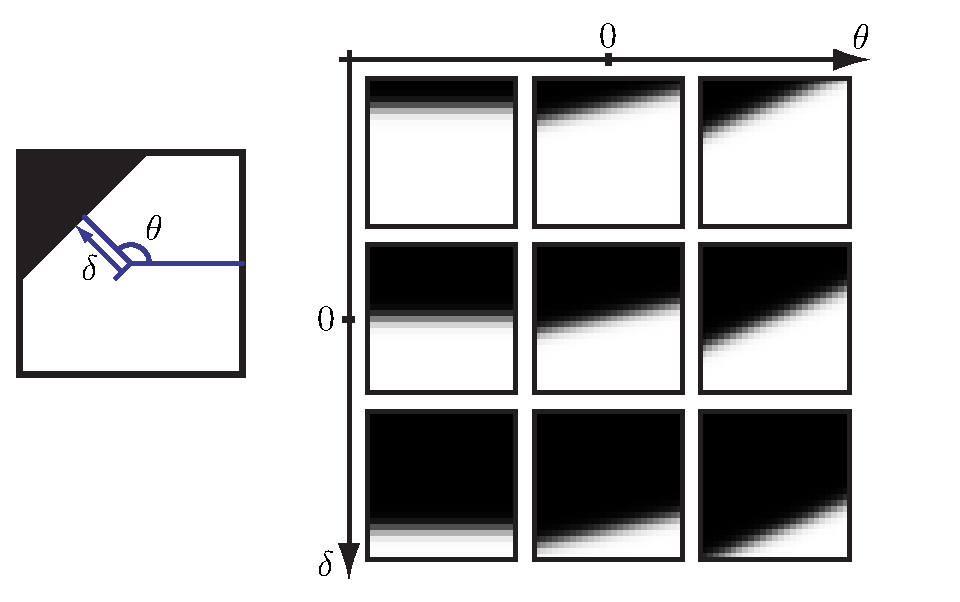
\includegraphics[width=0.55\linewidth]{edge-manifold.eps}
}{
Left: an example of cartoon image. Right: parameterization of the manifold of edge patches and some examples.
%
}{fig-edge-patches-samples}

For this simple class of black and white images, the set $\Mm$ is thus approximately sampled along a smooth manifold $\tMm$ of dimension 2 embedded in $\RR^{d}$ for $d=\tau^2$. In this case, the set $\Mm$ samples the whole continuous manifold $\tMm$, however this sampling might be highly non-uniform. The manifold $\tMm$ has the topology of a cylinder, and figure \ref{fig-edge-manifold} shows an example of a discrete set $\Mm$ sampled on this cylinder. 

\myfigure{
\raisebox{.3cm}{ %
\includegraphics[width=0.25\linewidth]{manifold/edges/cartoon-curves.png} }\qquad\qquad
\includegraphics[width=0.3\linewidth]{manifold/edges/cartoon-manifold.png}
}{
Left: a cartoon image. Right: 3D representation of the set $\Mm$ as samples of the edge manifold $\tMm$ (depicted in 3D as a cylinder). The two curves on the manifold corresponds to patches extracted along the two lines in the image.
%
}{fig-edge-manifold}


%%%%%%%%%%%%%%%%%%%%%%%%%%%%%%%%%%%%%%%%%%%%%%%%%%%%%%%%%%%%%%
%%%%%%%%%%%%%%%%%%%%%%%%%%%%%%%%%%%%%%%%%%%%%%%%%%%%%%%%%%%%%%
\section{Diffusions and Laplacians on a Manifold}

\label{subsec-diffusion-laplacians}

In order to process an image $f \in \ldeux(\La)$, this paper uses tools from graph theory and calculus on manifolds in order to modify the associated mapping $\lifted \in \ldeux(\Mm)$ defined over the discretized manifold $\Mm$. This section reviews several linear operators that can be applied to elements of $\ldeux(\Mm)$.

% In the following, we treat equivalently mappings $\lifted \in \ldeux(\Mm)$ and images $f \in \ldeux(\La)$ thanks to the association $\ldeux(\Mm) \simeq \ldeux(\La) \simeq \RR^n$.

%%%%%%%%%%%%%%%%%%%%%%%%%%%%%%%%%%%%%%%%%%%%%%%%%%%%%%%%%%
\subsection{Discrete Diffusion Operators on Graphs}
\label{subsect-discrete-diffusion}

% Following the manifold lifting exposed in section \ref{sec-highdim-lifting} we consider the lifted function $\manilift : \La \rightarrow \Mm$ defined in equation \eqref{eq-highdim-embedding}. 

In the three processing modes, the set $\Mm$ is embedded in the Euclidean space $\RR^{d}$ with $d = 2$ for local computations, $d=3$ for semi-local computations and $d=\tau^2$ for non-local computations. As shown in section \ref{subsect-manifold-structure}, in some special case, the set $\Mm$ is close to a low dimensional smooth manifold $\tMm$. It thus makes sense, for close enough features $p,q \in \Mm$ to consider their extrinsic distance $\norm{p-q}$ computed over $\RR^{d}$ as an approximation for the geodesic distance $d_{\tMm}(p,q)$ over $\tMm$ which is usually not available. 

\paragraph{Diffusion kernel}

In order to process a manifold mapping $g \in \ldeux(\Mm)$ (such as for instance $\lifted$ itself or other mappings), one defines a symmetric isotropic kernel on pairs of points of the discrete manifold
\begin{equation}
	\label{eq-defn-continuous-kernel}
	\foralls p,q \in \Mm, \quad W_0(p,q) \eqdef \exp\pa{ -\frac{\norm{p-q}^2}{2\si^2} }.
\end{equation}
The parameter $\si$ is supposed to be small enough so that the extrinsic computation of $\norm{p-q}$ approximates the geodesic distance $d_{\tMm}(p,q)$ for close pair of points $(p,q) \in \Mm^2$. In practice, $\si$  should be adapted for specific image processing applications. 

The normalized filtering kernel is defined as
\begin{equation}
	\label{eq-defn-continuous-normalization}
	W(p,q) \eqdef \frac{1}{D(p)} W_0(p,q) 
	\qqwhereqq
	D(p) \eqdef \sum_{q \in \La} W_0(p,q).
\end{equation}
The kernel $W$ defines an operator on mappings $g \in \ldeux(\Mm)$
\begin{equation}
	\label{eq-defn-diffusion}
	\foralls p \in \La, \quad W g(p) \eqdef 
	\sum_{p \in \Mm} W(p,q) g(q).
\end{equation}
This can be thought as a low-pass filtering of $g$ since this operator does not modify constant functions:  $W 1 = 1$. This filtering can be very different with respect to traditional isotropic filterings when one considers semi-local or non-local embeddings. The left images of figure \ref{fig-diffusion-graph} show the diffusion of a Dirac $W \delta$ located in the center of the image. This diffusion is performed using the operator $W$ corresponding to the three computation modes (local, semi-local and non-local). One should note that although $W \delta \in \ldeux(\Mm)$ is defined on the set $\Mm$, it can be equivalently displayed as a standard 2D image.

Linear operators such as $W$ acts on elements of $\ldeux(\Mm)$ which can be represented as discrete vectors in $\RR^n$ where $n=|\Mm|$ is the number of pixels in the input image $f$. These operators can thus be considered as $n \times n$ matrices.

\myfigure{
\hspace{0.18\linewidth}
\hspace{1mm}
\figitemraise{1.5cm}{a}
\includegraphics[width=0.18\linewidth]{diffusion/corral/corral-diffusion-local-3.png}
\includegraphics[width=0.18\linewidth]{diffusion/corral/corral-diffusion-local-4.png}
\includegraphics[width=0.18\linewidth]{diffusion/corral/corral-diffusion-local-5.png}
\includegraphics[width=0.18\linewidth]{diffusion/corral/corral-diffusion-local-6.png}\\\vspace{1mm}
\includegraphics[width=0.18\linewidth]{diffusion/corral/corral-original.png}
\hspace{1mm}
\figitemraise{1.5cm}{b}
\includegraphics[width=0.18\linewidth]{diffusion/corral/corral-diffusion-neigh-3.png}
\includegraphics[width=0.18\linewidth]{diffusion/corral/corral-diffusion-neigh-4.png}
\includegraphics[width=0.18\linewidth]{diffusion/corral/corral-diffusion-neigh-5.png}
\includegraphics[width=0.18\linewidth]{diffusion/corral/corral-diffusion-neigh-6.png}\\\vspace{1mm}
\hspace{0.18\linewidth}
\hspace{1mm}
\figitemraise{1.5cm}{c}
\includegraphics[width=0.18\linewidth]{diffusion/corral/corral-diffusion-un-normalized-3.png}
\includegraphics[width=0.18\linewidth]{diffusion/corral/corral-diffusion-un-normalized-4.png}
\includegraphics[width=0.18\linewidth]{diffusion/corral/corral-diffusion-un-normalized-5.png}
\includegraphics[width=0.18\linewidth]{diffusion/corral/corral-diffusion-un-normalized-6.png}
}{
Left: original image $f$.
Right: heat diffusions with an increasing time for: (a) local embedding $x \mapsto x$, (b) semi-local embedding $x \mapsto (x,\la f(x))$, (c) non-local embedding $x \mapsto p_x(f)$.
%
}{fig-diffusion-graph}

\paragraph{Laplacian operators}

The Laplacian operator $L$ and its symmetrized version $L_0$ are defined as 
\begin{equation}
	\label{eq-defn-laplacian}
	L \eqdef \Id - W \qqandqq 
	L_0 \eqdef D^{1/2} L D^{-1/2} = \Id - D^{-1/2} W_0 D^{-1/2},
\end{equation} 
where $D$ is the diagonal operator $D = \diag_{p \in \Mm}(D(p))$. 

The normalized Laplacian $L_0$ corresponds to a discrete graph Laplacian as defined for example by Chung \cite{chung-spectral-graph}. For computer graphics purposes, other discretizations of the Laplacian are available \cite{polthier-computational,xu-discrete-laplacian} that make use of a triangulation data-structure. On real image data-sets, finding such a triangulation is however non-trivial although some methods are emerging \cite{carlsson-topological}. 

% In practice, all current implementations of these manifold tools use only discrete graphs and does not extends to more complex data structures.

\paragraph{Gradient operators}

The gradient operator maps $g \in \ldeux(\Mm)$ defined on the discrete set $\Mm$ to a measure of similarity on each couple of points of $\Mm \times \Mm$
\begin{equation}
	\label{eq-dfn-gradient}
	\foralls (p,q) \in \Mm \times \Mm, \qquad
	(G g)(p,q) = \sqrt{W_0(p,q)} \pa{ \frac{g(p)}{\sqrt{D(p)}}-\frac{g(q)}{\sqrt{D(q)}}}.
\end{equation}
This gradient is thus a linear mapping $G : \ldeux(\Mm) \mapsto \ldeux(\Mm \times \Mm)$, which corresponds to a matrix of $n \times n^2$ elements. One can also consider point-wise gradient vectors
\eql{\label{eq-dfn-grad-vector}
	\foralls p \in \Mm, \quad G_p g = ( (G g)(p,q) )_{q \in \Mm},
}
which corresponds to vectors in $\RR^n$.

This normalized gradient is different from the more classical un-normalized gradient, as introduced for instance in \cite{gilboa-nonlocal-segmentation,gilboa-nonlocal-functionals}
\begin{equation}
	\label{eq-dfn-gradient-unnormalized}
	\foralls (p,q) \in \Mm \times \Mm, \qquad
	(\tilde G g)(p,q) = \sqrt{W_0(p,q)} \pa{ g(p)-g(q) }. 	
\end{equation}
Section \ref{subsect-numerical-comparison} and in particular figure \ref{fig-denoising-results-visual} studies the advantages of using the normalized formulation.

The Laplacian $L_0$ and its un-normalized version $D-W_0$ are symmetric operators than can be decomposed as
\begin{equation}
	\label{eq-decomposition-laplacian}
	L_0 = \transp{G} G
	\qqandqq
	D-W_0 = \transp{\tilde G} \tilde G
\end{equation}
where $\transp{G}$ is the transposed matrix.


\paragraph{Approximate Operators}

The diffusion and Laplacian kernels $W_0$ and $L_0$ are linear operators on $\ldeux(\Mm) \simeq \RR^n$ and are computed as matrices of size $n \times n$ acting on $\RR^n$. These matrices are defined using the gaussian weights \eqref{eq-defn-continuous-kernel} and are thus full and difficult to use for intensive computations. In order to speed up both filtering computations and eigenvectors extraction, one typically uses either a $k$-nearest-neighbors or an $\epsilon$-distance approximation of the gradient defined in equation \eqref{eq-dfn-gradient}
\begin{align}
	\label{eq-lowdim-approx-grad}
	(G^{k} g)(p,q) \eqdef &
	\left\{ 
	\begin{array}{cl}
		(G g)(p,q) & \text{if}\quad  q \in \text{NN}_k(p),\\
		0 & \text{otherwise,}
	\end{array}
	\right. \\
	\qqandqq
	(G^{\epsilon} g)(p,q) \eqdef &
	\left\{ 
	\begin{array}{cl}
		(G g)(p,q) & \text{if} \quad \norm{p-q} \leq \epsilon,	\\
		0 & \text{otherwise,}
	\end{array}
	\right.
\end{align}
where $q$ belongs to the set $\text{NN}_k(p)$ of $k$-nearest neighbors of $p$ if
\begin{equation*} 
	\#\enscond{r \in \Mm}{ \norm{p-r}<\norm{p-q} } < k.
\end{equation*}
The approximated Laplacians are defined as
\begin{equation}
	\label{eq-approximate-laplacian}
	L_0^k \eqdef \transp{G^k}G^k
	\qqandqq
	L_0^\epsilon \eqdef \transp{G^\epsilon}G^\epsilon.
\end{equation}
These reduced operators can be conveniently stored as sparse matrices which leads to efficient algorithms for the iterative resolution of partial differential equations and the extraction of eigenvectors. The convergence of $L_0^k$ and $L_0^\epsilon$ toward $L_0$ when $k \rightarrow n$ and $\epsilon \rightarrow 0$ is fast whenever the set of points $\Mm$ is close to a smooth manifold $\tMm$. The following section studies the convergence of these finite dimensional operators to their continuous counterparts when $n \rightarrow +\infty$.

%%%%%%%%%%%%%%%%%%%%%%%%%%%%%%%%%%%%%%%%%%%%%%%%%%%%%%%%%%
\subsection{Convergence Analysis}
\label{subsect-convergence-analysis}

In order to understand the behavior of the denoising algorithms proposed in this paper, it is important to study the connexion between the discrete operators introduced in section \ref{subsect-discrete-diffusion} and their continuous counterparts defined using differential calculus on manifolds.

As explained in section \ref{subsect-manifold-structure}, the set $\Mm$ can sometimes be well approximated by a low dimensional manifold $\tMm$. In order to study the convergence properties of operators such as $W$ and $L_0$, the discrete set $\Mm$ is supposed to be sampled on a continuous manifold $\tMm \subset \RR^{d}$ of dimension $\tilde d < d \ll n$. The Riemannian metric of $\tMm$ is defined thanks to the embedding of $\tMm$ in $\RR^d$.

For such a smooth manifold $\tMm$, the Laplace Beltrami $\Delta_{\tMm}$ operates on smooth functions $\tilde g \in \Ldeux(\tMm)$. It can be defined as the limit of a local averaging
\eql{\label{defn-cont-laplacian}
	\foralls p \in \tMm, \quad
	\frac{2}{\si^2}  \pa{ \tilde g(p) - (\Ww \tilde g)(p) }
	\quad\overset{\si \rightarrow 0}{\longrightarrow}\quad
	\Delta_{\tMm} \tilde g(p)
}
where $\Ww$ is a local geodesic averaging
\eql{\label{eq-geodesic-averaging}
	\foralls p \in \tMm, \quad
	(\Ww \tilde g)(p) = \frac{1}{|B(p)|} \int_{B(p)} \tilde g(q) \d q
	\qwhereq
	B(p) \eqdef \enscond{q \in \tMm}{ d_{\tMm}(p,q) \leq \si }
}
where $d_{\tMm}(p,q)$ is the geodesic distance along the manifold $\tMm$, the length of the shortest curve traced on $\tMm$ between $p$ and $q$.

Equation \eqref{defn-cont-laplacian} is a continuous version of the definition \eqref{eq-defn-laplacian} of the discrete Laplacians $L$ and $L_0$. The width $\si$ of the averaging in \eqref{eq-geodesic-averaging} is the equivalent of the width of the gaussian kernel in \eqref{eq-defn-continuous-kernel}. The discrete sum used in the avergaging \eqref{eq-defn-continuous-normalization} is replaced by a continuous averaging over a geodesic ball in \eqref{eq-geodesic-averaging}.

One can make this connection more precise since if the sampling $\Mm$ of $\tMm$ is uniform, both $L$ and $L_0$ converge to $\Delta_{\tMm}$. 
This convergence is proved by Belkin \cite{belkin-laplacian-eigenmaps} and Lafon \cite{coifman-geometric-diffusion} when one first take an infinite number of points and then $\si \rightarrow 0$. The following bound on both $n$ and $\si$ is derived by Singer \cite{singer-graph-manifold} and refines a result of Hein et al. \cite{hein-graph-to-manifold} in the case where $\Mm$ is drawn uniformly at random on $\tMm$
\eq{
	\forall p \in \Mm, \quad
	\frac{2}{\si^2} (L g)(p) = (\Delta_{\tMm} \tilde g)(p) + 
	O\pa{ n^{-1/2} \si^{ -(2+\tilde d/2) }, \si }.
}
where the discrete $g \in \ldeux(\Mm)$ is obtained by sampling a smooth function $\tilde g \in \Ldeux(\tMm)$.
The original bound \cite{singer-graph-manifold,hein-graph-to-manifold} is derived for $L$ but the result also applies to $L_0$.
This suggests an optimal asymptotic choice for the gaussian width $\si \eqdef C(\tMm) n^{-1/(6+\tilde d)}$, where $C(\tMm)$ is a constant that depends on geometric properties of $\tMm$. For this well chosen $\si$, the discrete Laplacians converges with a speed $\si$ toward $\Delta_{\tMm}$.

The main issue is thus to know wether, in applications to image processing, the set $\Mm$ is an uniform sampling of some continuous manifold $\tMm$. Indeed, this sampling is constrained by the lifting $x \in \La \mapsto \manilift(x) \in \Mm$, which might not be uniform in practical situations. To be more precise, one needs to make the distinction between the three modes of computation introduced in section \ref{sec-highdim-lifting}.
\begin{rs}
	\item  \textit{Local lifting:} in this case, the embedding is trivial $\manilift(x)=x$ and thus $L$ converges to 
	\eq{
		\Delta_{\tMm} = \Delta = -\pdd{}{x_1}-\pdd{}{x_2},
	}
	the traditional Laplacian over $\RR^2$. 
	\item \textit{Semi-local lifting:} in this case, $\Mm$ corresponds to a height field and $L$ is close to $\Ll$. If $\la$ in equation \eqref{eq-manifold-semi-local} is small, the sampling of the manifold is close to uniform. This approximate convergence is related to the convergence of neighboring filters to non-linear partial differential equations, see for instance \cite{barash-bilateral-pde,elad-bilateral,sochen-diffusion-confusion}
	\item \textit{Non-local lifting:} in this case, $\Mm$ might be a complicated set of points. Indeed, the examples of smooth images and cartoon images exposed in section \ref{subsect-manifold-structure} show that even in simple cases, this sampling might be far from uniform. In this case $L_0$ is very different from $\Ll$ and the convergence of $L_0$ to $\Delta_{\tMm}$ is not true in general. In some restricted cases one can however make an asymptotic derivation for non-local averaging operators, see for instance the analysis of the non-local means filter \cite{buades-pde}.
\end{rs}
 

%%%%%%%%%%%%%%%%%%%%%%%%%%%%%%%%%%%%%%%%%%%%%%%%%%%%%%%%%%%
\subsection{Manifold Spectral Basis}
\label{subsec-spectral-basis}

The symmetric Laplacian $L_0$ defined in equation \eqref{eq-defn-laplacian} is $L_0 = \Id - \tilde W$ where $\tilde W = D^{-1/2}W_0 D^{-1/2}$. Using the decomposition \eqref{eq-decomposition-laplacian}, the inner product associated to this symmetric operator can be written for $g  \in \ldeux(\Mm)$
\begin{equation*}
	\dotp{L_0 g}{g} = \dotp{\transp{G}G g}{g} = \dotp{G g}{G g} = \sum_{p,q \in \Mm} 
		W_0(p,q) \pa{ \frac{g(p)}{\sqrt{D(p)}}-\frac{g(q)}{\sqrt{D(q)}} }^2.
\end{equation*}
This implies that $L_0$ is a positive semi-definite operator with only the constant vectors in its kernel as soon as the graph is connected. One can thus define the orthogonal basis $(u_\om)_{\om = 0}^{n-1}$ of $\ldeux(\Mm)$
\eq{
	L_0 u_\om = \la_\om u_\om 
	\qqwithqq
	0 = \la_1 \leq \la_2 \leq \ldots \leq \la_n. 
}
These eigenvectors can be conveniently stored in an orthogonal matrix $U_0 \in \RR^{n \times n}$, where one uses the identification $\ldeux(\Mm) \simeq \RR^n$
\eq{
	\label{eq-laplacian-eigendec}
	U_0(p,\om) = u_\om(p)
	\qqarrqq
	L_0 = U_0 \La \transp{U_0} 
	\qwhereq
	\La = \{\la_\om\}_{\om}.
}
The parameter $\om$ plays the role of a frequency parameter with small $\om$ corresponding to low-frequencies. Indeed, in the case of the local lifting $\manilift(x)=x$, the eigenvectors of $L_0$ are exactly the Fourier basis, which can be written for the periodic 1D case as
\begin{equation}
	\label{eq-defn-eig-fourier}
	\foralls p \in \ZZ/n\ZZ, \quad
	\left\{
	\begin{array}{rcl}
	u_{2\om}(p) &=& \frac{2}{\sqrt{2n}}\cos\pa{ \frac{2\pi p \om}{n} },\\
	u_{2\om+1}(p) &=& \frac{2}{\sqrt{2n}}\sin\pa{ \frac{2\pi p \om}{n} },
	\end{array}
	\right.
	\qwithq
	\la_{2\om} = \la_{2\om+1} = \sin^2\pa{ \frac{\om\pi}{n} }.
\end{equation}
The eigendecomposition \eqref{eq-laplacian-eigendec} corresponds to the diffusion geometries expansion introduced by Coifman et al. \cite{coifman-geometric-diffusion} which has been applied to image graphs by Szlam et al. \cite{szlam-regularization}.

\myfigure{
\figitemraise{1.5cm}{a}
\includegraphics[width=0.22\linewidth]{diffusion/barb/barb-local-eigv-2.png}
\includegraphics[width=0.22\linewidth]{diffusion/barb/barb-local-eigv-11.png}
\includegraphics[width=0.22\linewidth]{diffusion/barb/barb-local-eigv-14.png}
\includegraphics[width=0.22\linewidth]{diffusion/barb/barb-local-eigv-16.png}\\\vspace{1mm}
\figitemraise{1.5cm}{b}
\includegraphics[width=0.22\linewidth]{diffusion/potatoe/potatoe-neigh-eigv-10.png}
\includegraphics[width=0.22\linewidth]{diffusion/potatoe/potatoe-neigh-eigv-19.png}
\includegraphics[width=0.22\linewidth]{diffusion/potatoe/potatoe-neigh-eigv-22.png}
\includegraphics[width=0.22\linewidth]{diffusion/potatoe/potatoe-neigh-eigv-25.png}\\\vspace{1mm}
\figitemraise{1.5cm}{c}
\includegraphics[width=0.22\linewidth]{diffusion/potatoe/potatoe-un-normalized-eigv-3.png}
\includegraphics[width=0.22\linewidth]{diffusion/potatoe/potatoe-un-normalized-eigv-5.png}
\includegraphics[width=0.22\linewidth]{diffusion/potatoe/potatoe-un-normalized-eigv-10.png}
\includegraphics[width=0.22\linewidth]{diffusion/potatoe/potatoe-un-normalized-eigv-11.png}
}{
Some eigenvectors $u_\om$ of Laplacians for
(a) the local Laplacian (Fourier basis),
(b) the semi-local Laplacian,
(c) the non-local Laplacian.
The image $f$ used to compute the discrete manifold is shown on figure \ref{fig-edge-patches-samples}, left.
%
}{fig-eigenvectors} 

%  as described in section \ref{sec-manifold-cartoon-images}
Figure \ref{fig-eigenvectors} shows some $u_\om$ on a cartoon image. It compares the eigenvectors of the local, semi-local and non-local Laplacians. The eigenvectors for the local Laplacian are the Fourier vectors that extend those of \eqref{eq-defn-eig-fourier} to 2D. The eigenvectors for the semi-local Laplacian are similar excepted that the oscillations are localized either inside or outside the boundary. The eigenvectors of the non-local Laplacian can be classified in three groups.
\begin{rs}
	\item The first two eigenvectors are constant on each side of the shape $B$. The projection on these two vectors recovers perfectly a binary cartoon image.
	\item The low frequency eigenvectors for small $\om$  are located along the boundary $\partial B$ and are highly oscillating. The projection on these eigenvectors recovers sharp steps along $\partial B$.
	\item The remaining higher frequencies are irrelevant and capture noise.
\end{rs}


%%%%%%%%%%%%%%%%%%%%%%%%%%%%%%%%%%%%%%%%%%%%%%%%%%%%%%%%%%%%%%
%%%%%%%%%%%%%%%%%%%%%%%%%%%%%%%%%%%%%%%%%%%%%%%%%%%%%%%%%%%%%%
%%%%%%%%%%%%%%%%%%%%%%%%%%%%%%%%%%%%%%%%%%%%%%%%%%%%%%%%%%%%%%
\section{Denoising: PDE Flows, Variational Minimization and Thresholding}

\newcommand{\energy}{\Ee}

Denoising is modeled in a probabilistic way as an inverse problem where one wishes to recover an image $f$ from a noisy observation $\F = \fz + \epsilon$ where $\epsilon$ is a white noise of variance $|\epsilon|^2$. A denoising algorithm builds an estimator $\bar f \in \RR^n$ of the true data $\fz$ that depends only on the observed $\F$. This estimator is a random vector that depends on the gaussian noise $\epsilon$ and its efficiency is measured using the expectation of the error $E(\norm{\fz-\bar f}^2)$. 

This section reviews three important classes of estimators, which are all based on taking advantage of a well chosen energy $\energy_{\F}(g)$ that should be small for typical images one wishes to recover. It is important to note that the energy $\energy_{\F}$ might depend on the noisy input $\F$ itself, which makes some of the proposed methods adaptive to the content of the image.

Sections \ref{sect-heat-diffusion-manifold}, \ref{sect-variational-regularization} and \ref{sec-thresholding} specialize these three kinds of estimators to computations on a discrete manifold $\Mm$. They use either operators such as the gradient and the Laplacian on $\Mm$ (defined in section \ref{subsect-discrete-diffusion}) or the manifold spectral basis (introduced in section \ref{subsec-spectral-basis}) to define the energy $\energy_{\F}$. 

Two approaches are usually considered in the literature. The first one uses tools from variational calculus and partial differential equations, while the other one exploits decompositions of harmonic analysis with thresholdings in orthogonal bases. All the proposed estimators $\bar f = \F_t$ depend on some scale $t>0$ that controls the degree of regularization one imposes on the solution. This scale is adapted to the noise level more or less automatically.


%%%%%%%%%%%%%%%%%%%%%%%%%%%%%%%%%%%%%%%%%%%%%%%%%%%%%%%%%%%%%%
\subsection{PDE Flows}
\label{subsect-pde-flows}

A PDE-flow regularizes the original noisy input $\F$ by a gradient descent of the energy
\eql{\label{eq-pde-flow}
	\foralls t>0, \quad \pd{\F_t}{t} = - \text{grad}_{\F_t} (\energy_{\F})
	\qqwithqq \F_0=\F.
}
If the original energy $\energy_{\F}$ is quadratic, this leads to a linear differential equation, otherwise it can be non-linear. For instance, the heat equation and the total variation flow are derived formally from 
\eq{
	\energy_{\F}(f) = 
	\choice{
		\frac{1}{2} \int |\nabla_x f|^2 \d x,\\
		\int |\nabla_x f| \d x
	}
	\qarrq
	\pd{\F_t^{\heat}}{t}(x) =
	\choice{
		\Delta \F_t\\
		\div\pa{ \frac{\nabla \F_t}{\norm{\nabla \F_t}} }
	}
}
and do not depend on $\F$. Other non-linear flows such as the anisotropic diffusion of Perona and Malik \cite{perona-anisotropic} can be considered. 

It is also possible to compute quadratic energies that depend on $\F$, such as an anisotropic diffusion along a tensor field estimated from $\F$, see \cite{weickert-coherence}. In this case, although the flow $t \mapsto \F_t$ is linear, the estimator computation $\F \mapsto \F_t$ is actually non-linear because $\energy_{\F}$ depends on the noisy input $\F$. Section \ref{sect-heat-diffusion-manifold} derives PDE flows using an energy $\energy_{\F}$ computed using operators on the discrete manifold $\Mm$. Such energies depends on $\F$ and makes the whole computation adaptive and non-linear.

\paragraph{Time-dependant manifold}

The flow of equation \eqref{eq-pde-flow} is computed from the energy $E_{\F}$ which depends only on the noisy input image. The discrete manifold $\Mm$ is computed once for all from the original input and does not change during the computations. Another option is to modify the manifold and actually compute it from the current estimate $\F_t$ at time $t$
\eql{\label{eq-time-dtp-flow}
	\foralls t>0, \quad \pd{\F_t}{t}(x) = - \text{grad}_{\F_t} (\energy_{\F_t})
	\qqwithqq \F_0=\F.
}
The overall process becomes even more non-linear than the original PDE.

Several works on adaptive filtering use such time-dependant regularization, see for instance anisotropic diffusion along time-varying tensors fields \cite{tschumperle-inpainting} and diffusion on triangulated surfaces~\cite{desbrun-implicit-fairing}.

%%%%%%%%%%%%%%%%%%%%%%%%%%%%%%%%%%%%%%%%%%%%%%%%%%%%%%%%%%%%%%
\subsection{Variational Regularization}
\label{subsect-variational-regularization}

A variational regularization defines an estimator $\F_t$ as a minimizer of a penalized functional
\begin{equation} % ^{\text{T}}
	\label{eq-variational-regularization}
	\foralls t\geq 0, \qquad \F_t = \uargmin{g} \frac{1}{2} \norm{\F-g}_{\ldeux}^2 + t \energy_{\F}( g ),
\end{equation}
The Rudin-Osher-Fatemi denoising method \cite{rudin-tv} for instance uses the total variation energy $\energy(g) \eqdef \int \abs{\nabla g}$ which does not depend on $\F$. 


%%%%%%%%%%%%%%%%%%%%%%%%%%%%%%%%%%%%%%%%%%%%%%%%%%%%%%%%%%%%%%
\subsection{Thresholding in an Orthogonal Basis}
\label{subsect-thresholding-ortho-basis}

Another line of research, initiated by Donoho and Johnstone \cite{donoho-shrinkage}, solves the estimation problem using operators that manipulate independently each coefficient of the decomposition of $\F$ in an orthogonal basis. 

\paragraph{$\ldeux$, $\lun$ and $\lzero$ regularization}

Thresholding operators in an orthogonal basis $\{u_\om\}_\om$ of $\RR^n$ are defined as
\begin{equation}
	\label{eq-thresh-estimator}
	\F_t^p \eqdef \sum_\om s_t^p(\dotp{\F}{u_\om}) \, u_\om
	\qqforqq p \in \{0,1,2\}.
\end{equation}
The pointwise functional $s_t^p$ modifies independently each coefficient and is defined by
\begin{align*}
	s_t^2(x) = \frac{x}{1+t \la_\om},
	\qquad
	s_t^1(x) & \eqdef
	\left\{
	\begin{array}{lll}
		x-\text{sign}(x)t & \text{if} & |x| > t,\\
		0 & \text{if} & |x| \leq t,
	\end{array}
	\right.\\
	\qqandqq
	s_t^0(x) & \eqdef 
	\left\{
	\begin{array}{lll}
		x & \text{if} & |x| > t,\\
		0 & \text{if} & |x| \leq t.
	\end{array}
	\right.
\end{align*}
The estimator $\F_t^2$ is linear and depends on a set of weights $\la_\om>0$ whereas the soft thresholding $\F_t^1$ and hard thresholding $\F_t^0$ perform a non-linear denoising. 

In order to achieve an optimal decay rate of the risk $E(\norm{\fz-\F_t})$, Donoho and Johnstone \cite{donoho-shrinkage} shows that one can use the universal threshold value $t \eqdef |\epsilon|\sqrt{2\log(n)}$. In practice however this threshold value can be set approximately to $t = 3 |\epsilon|$.

These estimators enjoy several optimality results when the function $\fz$ to recover belongs to a smoothness class that can be efficiently approximated linearly (for $p=2$) or non-linearly (for $p=1$ and $p=0$). Donoho and Johnstone \cite{donoho-shrinkage} show that $\F_t^0$ and $\F_t^1$, for the universal threshold $t \eqdef |\epsilon|\sqrt{2\log(n)}$, are asymptotically minimax for the estimation of piecewise regular 1D signals when one uses the wavelet basis \cite{mallat-book}. 


\paragraph{Variational interpretation of thresholding}

As shown by \cite{chambole-variational-wavelets}, these thresholding operators are also minimizers of variational energies of the form \eqref{eq-variational-regularization} 
\eql{\label{eq-variational-thresholding}
	\F_t^p = \uargmin{g} \frac{1}{2} \norm{\F-g}_{\ldeux}^2 + t \energy_{\F}^p( g )
	\qwhereq
	\choice{
		\energy_{\F}^2(g) = \frac{1}{2} \sum_\om \la_\om \abs{\dotp{g}{u_\om}}^2, \\
		\energy_{\F}^1(g) = \sum_\om \abs{\dotp{g}{u_\om}},\\
		\energy_{\F}^0(g) = \frac{t}{2} \#\enscond{ \om }{ \dotp{\F}{u_\om} \neq 0 }.
	}
}
This bridges the gap between the construction of variational denoisers and the use of orthogonal bases. 

If the orthogonal basis $(u_\om)_\om$ is a fixed basis (such as Fourier or wavelets) then the energy $\energy_{\F}^p$ do not depends on the input $\F$ and the estimator $\F_t$ is non adaptive. Section \ref{sec-thresholding} uses manifold spectral bases computed from $\F$, which makes the thresholding estimators adaptive to the input.


% optimized and thresholding \eqref{eq-variational-thresholding} leads to numerical results similar to PDE-based formulations \eqref{eq-variational-regularization}.

% This universal threshold shows that thresholding in orthogonal bases are usually simpler to set-up in denoising applications.

% The threshold value $T$ should be set just below the noise level $|\epsilon|$ in order to remove all the noisy coefficients $\dotp{\epsilon}{u_\om}$ that are gaussian random variable of variance $|\epsilon|^2$. Asymptotically, the optimal value for this threshold is $T \eqdef |\epsilon|\sqrt{2\log(n)}$, see \cite{donoho-shrinkage}.



%%%%%%%%%%%%%%%%%%%%%%%%%%%%%%%%%%%%%%%%%%%%%%%%%%%%%%%%%%%%%%
%%%%%%%%%%%%%%%%%%%%%%%%%%%%%%%%%%%%%%%%%%%%%%%%%%%%%%%%%%%%%%
%%%%%%%%%%%%%%%%%%%%%%%%%%%%%%%%%%%%%%%%%%%%%%%%%%%%%%%%%%%%%%
\section{Filtering and Diffusion on Manifolds}
\label{sect-heat-diffusion-manifold}

This section explains how PDE flows introduced in section \ref{subsect-pde-flows} can be extended by using energies $\energy_{\F}$ derived from operators on the manifold set $\Mm$. Such energies are used to process the function $\tf \in \ldeux(\Mm)$ defined from the noisy input $f \in \ldeux(\La)$, see equation \eqref{eq-def-lifted}. Since the set $\Mm = (\manilift(x))_x$ is computed from the noisy input $\F$, the corresponding flow $t \mapsto \F_t$ is adaptive and non-linear even if $\energy_{\F}$ is a quadratic energy. One recovers this way several recently proposed semi-local and non-local denoising algorithms. 

% such as the non-local means \cite{buades-nl-means} and diffusion maps with the heat equation on graphs \cite{szlam-regularization}.

% Originally, operators such as averaging $W$ (defined in equation \eqref{eq-defn-continuous-normalization}), Laplacian $L_0$ (defined in equation \eqref{eq-defn-laplacian}) or gradient (defined in equation \eqref{eq-dfn-gradient}) are applied to elements of $\ldeux(\Mm)$. In the following, they are applied to images in which are vectors $g \in \RR^n$ thanks to the identification $\ldeux(\Mm) \simeq \RR^n$ given by the lifting $\manilift$ between pixels in $\La$ and elements of $\Mm$.


% filtering and PDE diffusion is extended to the graph setting in order to construct various estimators. 

%%%%%%%%%%%%%%%%%%%%%%%%%%%%%%%%%%%%%%%%%%%%%%%%%%%%%%%%%%%%%%
\subsection{Non-iterative Manifold Smoothing}
\label{sect-noniterative-smoothing}

Before introducing linear and non-linear PDE flows, a simpler approach to denoise $\F$ is to perform a 1-step diffusion of $\tf \in \ldeux(\Mm)$
\begin{equation}
	\label{eq-noniterative-diffusion}
	\F_t \eqdef W \tF,
\end{equation} 
using the averaging operator defined in equation \eqref{eq-defn-continuous-normalization}. The scale parameter $t$ of this estimator corresponds to the scale $t=\si$ used in the definition of the smoothing kernel \eqref{eq-defn-continuous-kernel}.

To minimize the average risk $E(\norm{\F_t-\tilde \fz}^2)$, one needs to correctly define this scale parameter $t$ that should grow in proportion to the noise level $|\epsilon|$. This non-iterative denoising approach corresponds to various filtering operators.
\begin{rs}
	\item An isotropic linear filtering for the local embedding $\manilift(x)=x$: the operator $W$ is a convolution against a gaussian kernel.
	\item A spatially varying filter for the semi-local embedding $\manilift(x)=(x,\la \F(x))$: the degree of spatial adaptivity is controlled by $\la$ and the corresponding filter $y \mapsto W(x,y)$ is compactly supported around $x$. In a general setting, the corresponding estimator can be written as
	\eq{
		\bar f(x) = \frac{1}{D(x)} \sum_{y} 
			w_{\text{s}}\pa{ \frac{\norm{x-y}}{\si_{\text{s}}} }
			w_{\text{v}}\pa{ \frac{\norm{\F(x)-\F(y)}}{\si_{\text{v}}} } \F(y)
	}
	where $D(x)$ is the usual normalizing term. 
	Our choice of gaussian weight \eqref{eq-defn-continuous-kernel} corresponds to choosing $w_{\text{s}} = w_{\text{v}}$ as a gaussian kernel and $\si_{\text{s}}/\si_{\text{v}} = \la$ is the embedding constant. Depending on specific choice for $w_{\text{s}}$ and $w_{\text{v}}$, one retrieve several neighborhood filters such as Yaroslavsky's filter \cite{yaroslavsky-book}, the bilateral filter \cite{tomasi-bilateral} or Susan filter \cite{smith-susan}.
	\item A spatially non-local filter for the non-local embedding $\manilift(x)=p_x(\F)$: this corresponds to the non-local means of Buades et al. \cite{buades-nl-means}. In a general setting, the corresponding non-local estimator can be written as
	\eq{
		\bar f(x) = \frac{1}{D(x)} \sum_{y} 
			w\pa{ \frac{\norm{p_x(\F)-p_y(\F)}}{\si} } \F(y)
	}
	where $D(x)$ is the usual normalizing term. Our choice of gaussian weight \eqref{eq-defn-continuous-kernel} corresponds to the original choice of $w$, see \cite{buades-nl-means}, but other kernels can be used. 	
	More advanced non-local filters have been also proposed, see for instance \cite{dabov-collaborative-filtering}.
\end{rs} 
It is important to note that, although the filtering $\tF \mapsto W \tF$ is linear, the operator $W$ depends in a non-linear way on the input $\F$, making the overall process non-linear.


%%%%%%%%%%%%%%%%%%%%%%%%%%%%%%%%%%%%%%%%%%%%%%%%%%%%%%%%%%%%%%
\subsection{Manifold Heat Diffusion}
\label{sect-heat-diffusion}

Instead of performing a fixed amount of diffusion, one can consider a continuous diffusion process defined through the normalized gradient $L$ defined in equation \eqref{eq-dfn-gradient}. This heat diffusion corresponds to the PDE flow \eqref{eq-pde-flow} of the following manifold quadratic energy
\eql{\label{eq-quadratic-gradient}
	\foralls g \in \ldeux(\Mm), \quad
	\energy_{\F}^{\quadra}(g) = \frac{1}{2}\norm{G g}^2,
}
which depends on the input $\F$ since the operator $G$ is computed on the discrete manifold $\Mm$.

To diffuse a noisy image $\F$, one thus looks for a function $(x,t) \mapsto \F_t^{\heat}(x)$ that satisfies
\begin{equation}\label{eq-heat-diffusion}
	\foralls t>0, \quad \pd{\F_t^{\heat}}{t}(x) = -L \F_t^{\heat}(x)
	\qqwithqq \F_0^{\heat} = \tF.
\end{equation}
The estimator of $\fz$ from the noisy data $\F$ is then defined as $\F_{t}^{\heat}$ where the stopping time $t$ should be carefully chosen to match the noise level $|\epsilon|$.

It is important to note that in this application, the width $\si$ of the smoothing kernel $W_0$, equation  \eqref{eq-defn-laplacian}, is independent of the noise level $|\epsilon|$. This width $\si$ should be set to account for the sampling $\Mm$ of the true underlying continuous manifold. This is different from the non-iterative diffusion \eqref{eq-noniterative-diffusion} where $\si$ depends on $|\epsilon|$.

The PDE \eqref{eq-quadratic-gradient} is applied to a discrete manifold in the geometric diffusion framework \cite{coifman-geometric-diffusion}. It has been used to process images with semi-local and non-local embeddings by Szlam et al. \cite{szlam-regularization}. The mean-shift procedure with a gaussian kernel applied to the set $\Mm$ as done \cite{comaniciu-mean-shift} is closely related to \eqref{eq-quadratic-gradient}. This diffusion is also related to the short time evaluation of the Laplace Beltrami flow of Spira et al. \cite{spira-short-time-beltrami}, although these procedures correspond to a time-dependant embedding and a PDE diffusion flow (see the end of section \ref{subsect-pde-flows}).

\paragraph{Iterative resolution}

The equation \eqref{eq-heat-diffusion} can be solved using an explicit discretization in time with time-steps $\eta$. This leads to the following iterations
\begin{equation}
	\label{eq-iterative-heat-eq}
	\F_{k+1}^{\heat} = (1-\eta)\F_k^{\heat} + \eta W \F_k^{\heat} \qqwithqq \F_0^{\heat}=\tF. 
\end{equation}
If one chooses $\eta=t/k$, one has $\F_{k}^{\heat} \rightarrow \F_t^{\heat}$ when $k \rightarrow +\infty$. To ensure numerical stability, $n$ and $k$ should grow according to the CFL condition. The non-iterative denoising, equation \eqref{eq-noniterative-diffusion}, corresponds to only one iteration of this process with a large time step $\eta=1$.

\myfigure{
\begin{tabular}{ccc}
\includegraphics[width=0.25\linewidth]{diffusion/barb/img/barb-denoising-local-1.png}&
\includegraphics[width=0.33\linewidth]{diffusion/barb/barb-denoising-local-coefficients.png} &
\includegraphics[width=0.33\linewidth]{diffusion/barb/barb-denoising-neigh-coefficients.png} \\
Image $\tF$ & Local embedding & Non-local embedding
\end{tabular}
}{
The coefficients $|\dotp{\tF}{u_\om}|$ of a noisy image $\F$.
Center: using the local spectral basis $(u_\om)_\om$, which is the Fourier basis, right: using the non-local spectral basis.
%
}{fig-eigendecomposition} 

\paragraph{Spectral resolution}

The normalized Laplacian introduced in equation \eqref{eq-defn-laplacian} is related to the symmetric Laplacian through $L = D^{-1/2} L_0 D^{1/2}$. The eigenvectors of $L$ are thus $U = D^{-1/2} U_0$ and one can compute the eigendecomposition of some vector $g$ on $U$ as 
\begin{equation*}
	\hat g(\om) = (U^{-1}g)(\om) = \dotp{u_\om}{D^{1/2} g}.
%	\qqwhereqq
%	U^{-1} g = \transp{U_0} D^{1/2} g.
\end{equation*}
This spectral decomposition $\hat g$ allows one to solve the heat equation in the transformed domain since
\begin{equation}
	\label{eq-spectral-atenuation}
	\foralls \om, \quad \frac{\d}{\d t} \hat \F_t^{\heat}(\om) = -\la_\om \hat \F_t^{\heat}(\om)
	\qquad\Longrightarrow\qquad
	\hat \F_t^{\heat}(\om) = e^{-\la_\om t} \hat \tF(\om).
\end{equation}
This equation allows one to solve exactly for $\F_t^\heat$ and offers a non-iterative alternative to \eqref{eq-iterative-heat-eq} to compute the solution of the heat equation at a fixed time $t$. The diffused function $\F_t^{\heat}$ at a time $t$ has its spectral coefficients reduced by the factor $e^{-\la_\om t}$ which is small for large $t$ and for high-frequencies $\om$. 

On figure \ref{fig-eigendecomposition}, one can see the magnitude of noisy coefficients $\dotp{\tF}{u_\om}$ for the local and non-local expansions. The energy of the image is more concentrated on the low frequency part of the spectrum for the non-local Laplacian. This is a result of the adaptivity of the non-local Laplacian to the geometric content of the image. The high frequency residual is mostly the projection of the noise $\dotp{\tilde \epsilon}{u_\om}$. This compaction of the energy makes the heat diffusion over the non-local manifold much more efficient that over the local one, since the spectral attenuation efficiently removes the high frequency noise.


\paragraph{Diffusion examples}

Figure \ref{fig-diffusion-graph} shows the filtering $\F_t^{\heat}$ of an impulse Dirac distribution $\F_0^{\heat}=\delta$. On figure \ref{fig-heat-flow} one can see the time evolution of $\F_t^{\heat}$ for the three computation modes, starting from the noisy input $\F_0^{\heat} = \tF$.
\begin{rs}
	\item The local embedding leads to the traditional Euclidean heat equation. This diffusion blurs the image since the embedding does not take into account the geometric features of $f$.
	\item Both the semi-local and the non-local embeddings correspond to a non-linear processing of $\F$ since the Laplacian $L$ takes into account the structures of the image. This leads to a diffusion that does not blur the geometrical features. On geometrical images, these two diffusions give similar results. On complex natural images, non-local diffusion often surpasses semi-local diffusion as reported by Buades et al. \cite{buades-nl-means}, see section \ref{sec-numerical-results}. % It is however beyond the scope of this paper to study in details the performances of non-linear heat equations for denoising scenarios.
\end{rs}

\myfigure{
\figitemraise{1.5cm}{a}
\includegraphics[width=0.22\linewidth]{diffusion/barb/img/barb-denoising-local-1.png}
\includegraphics[width=0.22\linewidth]{diffusion/barb/img/barb-denoising-local-3.png}
\includegraphics[width=0.22\linewidth]{diffusion/barb/img/barb-denoising-local-5.png}
\includegraphics[width=0.22\linewidth]{diffusion/barb/img/barb-denoising-local-6.png}\\\vspace{1mm}
\figitemraise{1.5cm}{b}
\includegraphics[width=0.22\linewidth]{diffusion/barb/img/barb-denoising-neigh-1.png}
\includegraphics[width=0.22\linewidth]{diffusion/barb/img/barb-denoising-neigh-3.png}
\includegraphics[width=0.22\linewidth]{diffusion/barb/img/barb-denoising-neigh-5.png}
\includegraphics[width=0.22\linewidth]{diffusion/barb/img/barb-denoising-neigh-6.png}\\\vspace{1mm}
\figitemraise{1.5cm}{c}
\includegraphics[width=0.22\linewidth]{diffusion/barb/img/barb-denoising-un-normalized-1.png}
\includegraphics[width=0.22\linewidth]{diffusion/barb/img/barb-denoising-un-normalized-3.png}
\includegraphics[width=0.22\linewidth]{diffusion/barb/img/barb-denoising-un-normalized-4.png}
\includegraphics[width=0.22\linewidth]{diffusion/barb/img/barb-denoising-un-normalized-5.png}
}{
Heat flow $\F_t^{\heat}$ with an increasing $t$ for: (a) local embedding (traditional heat equation)
(b) semi-local embedding, (c) non-local embedding. 
%
}{fig-heat-flow}


%%%%%%%%%%%%%%%%%%%%%%%%%%%%%%%%%%%%%%%%%%%%%%%%%%%%%%%%%%%%%%
\subsection{Time-dependant Manifold Diffusion}
\label{sect-time-dpt-manifold}

The manifold diffusion \eqref{eq-heat-diffusion} use a fixed discrete manifold $\Mm$ computed from the noisy input $\tF$. As defined in equation \eqref{eq-time-dtp-flow}, it is possible to consider a flow where the manifold is continuously updated during the diffusion
\eql{\label{eq-time-dtp-manifold-flow}
	\foralls t>0, \quad \pd{\F_t^{\tilde \heat}}{t}(x) = -L_{\Mm_t} \F_t^{\tilde \heat}(x)
	\qqwithqq
	\choice{
		 \F_0^{\tilde \heat} = \tF,\\
		 \Mm_t = \pa{ \phi_{ \F_t^{\tilde \heat} }(x) }_{x \in \La}
	}
}
In this equation, the manifold $\Mm_t$ is computed from the solution of flow at time $t$, and the dependancy of the Laplacian operator $L=L_{\Mm_t}$ on the manifold is made explicit. The resulting flow $t \mapsto \F_t^{\tilde \heat}$ depends non-linearly from the initial condition $\F_0^{\tilde \heat}$, which makes the overall process radically different from the original heat flow $\F_t^{\heat}$.

Such a time-dependant flow has been defined, in the semi-local setting, by Spira et al. \cite{spira-short-time-beltrami}, where the Laplacian is an accurate discretizeation of the Laplace Beltrami $\Delta_{\tMm}$ of the height field $\tMm$. In the non-local setting, this flow shares similarities with iterated non-local means filterings introduced by Brox and Cremers \cite{brox-iterated-nl-means}. This iterated non-local means however does not converge to $\F_t^{\tilde \heat}$ but rather to a stationary point of a filtering process.

The non-linear PDE \eqref{eq-time-dtp-manifold-flow} can be solved explicitly in time by iterating the following two steps
\eq{
	\choice{
	\Mm_k = \pa{ \phi_{ \F_{k}^{\tilde \heat} }(x) }_{x \in \La}, \\
	\F_{k+1}^{\tilde \heat} = (1-\eta)\F_k^{\tilde \heat} + \eta W_{\Mm_k} \F_k^{\tilde \heat}, 
	}
}
with the initialization $\F_0^{\tilde \heat} = \tF$ and where the averaging $W_{\Mm_k}$ is computed using the discrete manifold $\Mm_k$.


%%%%%%%%%%%%%%%%%%%%%%%%%%%%%%%%%%%%%%%%%%%%%%%%%%%%%%%%%%%%%%
%%%%%%%%%%%%%%%%%%%%%%%%%%%%%%%%%%%%%%%%%%%%%%%%%%%%%%%%%%%%%%
%%%%%%%%%%%%%%%%%%%%%%%%%%%%%%%%%%%%%%%%%%%%%%%%%%%%%%%%%%%%%%
\section{Variational Regularization on Manifolds}
\label{sect-variational-regularization}

As explained in section \ref{subsect-variational-regularization}, one can replace the PDE flow by a variational optimization that takes into account both a regularization through the energy $\energy_{\F}$ and an attach to the original noisy data. 

This section first details the quadratic energy \eqref{eq-quadratic-gradient} in the case of a discrete manifold energy $\energy_{\F}$ and then proposes other non-linear alternatives. These estimators have been proposed in recent works using a slightly different formalism. We show how they fit into the regularization framework introduced in section \ref{subsect-variational-regularization} and detail several algorithms to compute efficiently these flows.

%%%%%%%%%%%%%%%%%%%%%%%%%%%%%%%%%%%%%%%%%%%%%%%%%%%%%%%%%%%%%%
\subsection{Quadradic Manifold Regularization}
\label{subsect-quad-regularization}

The quadratic energy \eqref{eq-quadratic-gradient} used to define the heat equation leads to the following quadratic regularization 
\eql{
	\label{eq-quadr-regul}
	\foralls t\geq 0, \qquad \F_t^{\quadra} = \uargmin{g \in \ldeux(\Mm)} \norm{\tF-g}_{\ldeux}^2 + t \norm{ G g }_{\ldeux}^2
}
where the manifold gradient $G$ is defined in equation \eqref{eq-dfn-gradient}. 

A similar energy is studied by Gilboa and Osher for image restoration and segmentation \cite{gilboa-nonlocal-segmentation}. They use a continuous formulation of the non-normalized gradient $\tilde G$ as defined in equation \eqref{eq-dfn-gradient-unnormalized}, whereas in this paper we use a normalized operator $G$ defined in equation \eqref{eq-defn-laplacian}. For semi-supervised learning applications, Belkin et al. \cite{belkin-manifold-regularization} have introduced a manifold regularization framework that performs interpolation by a quadratic penalization similar to \eqref{eq-quadr-regul}.

Once the operator $G$ is fixed, the solution of minimization \eqref{eq-quadr-regul} depends linearly on the input $\F$ and requires the inversion of the graph laplacian $L_0 = \transp{G}G$
\begin{equation*}
	\foralls t\geq 0, \qquad \F_t^{\quadra} = (\Id+t \transp{G}G)^{-1} \tF = (\Id+t L_0)^{-1} \tF.
\end{equation*}
It is important to remember that the mapping $\F \mapsto \F_t^{\quadra}$ is however non-linear because $G$ actually depends on $\F$ in a non-linear way.

One can take advantage of the spectral basis introduced in equation \eqref{eq-laplacian-eigendec} and compute the quadratic regularized solution over the transformed domain
\begin{equation*}
	\foralls t\geq 0, \qquad 
	\dotp{\F_t^{\quadra}}{u_\om} = \frac{1}{1+t\la_\om} \dotp{\tF}{u_\om}. 
\end{equation*}
One should compare this spectral attenuation with the one obtained in \eqref{eq-spectral-atenuation} for the heat equation. The diagonal kernel for the quadratic regularization is $(1+t\la_\om)^{-1}$ which is similar to the low-pass kernel  $e^{-\la_\om t}$ of the heat diffusion. 

This quadratic regularization \eqref{eq-spectral-atenuation} can also be interpreted as an estimator $\F_t^2$ as described in equation \eqref{eq-variational-thresholding} using the spectral basis $\{u_\om\}_\om$ and the eigenvalues $\la_\om$ as quadratic weights.

% It is however important to note that in this setting, $\F_t^2$ does not depend linearly on $\F$ since the spectral basis $\{u_\om\}_\om$ depends non-linearly on $\F$ through the construction of the manifold graph.

 
%%%%%%%%%%%%%%%%%%%%%%%%%%%%%%%%%%%%%%%%%%%%%%%%%%%%%%%%%%%%%%
\subsection{Total Variation Manifold Regularization}
\label{subsect-total-variation-graph}

In order to turn the quadratic regularization \eqref{eq-quadr-regul} into a non-linear penalty that favors emergence of large gradients near discontinuities, one can consider the following non-linear TV-like energy
\eq{
	\foralls g \in \ldeux(\Mm), \quad
	\energy_{\F}^{\tv}(g) = \sum_{p \in \Mm} \norm{G_p g}_{\ldeux},
}
where the gradient vector $G_p g$ is defined in equation \eqref{eq-dfn-grad-vector}.
The estimator is defined as
\begin{equation}
	\label{eq-nonlocal-tv}
	\F_t^{\tv} = \uargmin{g \in \ldeux(\Mm)} \frac{1}{2}\norm{\tF-g}_{\ldeux}^2 + t 
	\sum_{p \in \Mm} \norm{ G_p g }.
\end{equation}
A similar formulation is introduced by Gilboa et al. \cite{gilboa-nonlocal-functionals} in the continuous setting. They use the un-normalized Laplacian introduced in equation \eqref{eq-dfn-gradient-unnormalized} whereas our formulation \eqref{eq-nonlocal-tv} uses the normalized gradient \eqref{eq-dfn-gradient}. Section \ref{subsect-numerical-comparison} and in particular figure \ref{fig-denoising-results-visual} shows the superiority of the normalized regularization over regular areas of the image. A related non-linear energy is used in Kindermann et al. \cite{kindermann-nonlocal-functionals} to solve more general inverse problems. An alternative non-linear regularization is proposed by  Zhou and Sch\"{o}lkopf \cite{zhou-regularization-discrete} and Elmoataz et al. \cite{elmoataz-nonlocal} that consider the $p$-laplacian which is non-linear for $p \neq 2$.

The estimator $\F_t^{\tv}$ depends non-linearly on the input $\F$ both because the energy $\energy_{\F}^{\tv}$ is not quadratic and because the operator $G$ depends non-linearly on $\F$.
The computation of $\F_t^{\tv}$ requires some special care for points $p$ where $G_p \F_t^{\tv}$ is small. A simple fix consists in replacing $\energy_{\F}^{\tv}$ by a regularized functional such as
\eq{
	\energy_{\F}^{\tv,\eta}(g) = 
	\sum_{p \in \Mm} (\eta^2 + \sum_q \abs{ (G g)(p,q)}^2)^{1/2}
} 
for a small enough $\eta$. A more accurate approach solves the discrete optimization problem with the help of the graph-cut algorithm~\cite{gilboa-nonlocal-functionals}.

In this paper we propose to solve the non-linear problem \eqref{eq-nonlocal-tv} using an iterative scheme derived from Chambole's algorithm~\cite{chambolle-algo-tv} originally designed to solve the classical Rudin-Osher-Fatermi flow~\cite{rudin-tv}. The algorithm iteratively computes gradient fields $\th^k = (\th^k(p))_p$, where each $\th^k(p)$ is a vector in $\RR^n$. The algorithm initially set 
\eq{
	\foralls p \in \Mm, \quad \th^0(p) = 0 \in \RR^n
} 
and iterates
\begin{equation*}
	\foralls p \in \Mm, \quad
	\th^{k+1}(p) = \frac{ \th^k(p) - \eta g(p) }{1+\eta \norm{g(p)}}
	\qwhereq
	g = G ( \transp{G} \th^k - \tF/t ).
\end{equation*}
One can then prove \cite{chambolle-algo-tv} that if $\eta$ is small enough, 
\begin{equation*}
	\tF-t\transp{G} \th^k 
	\;\overset{k \rightarrow +\infty}{\longrightarrow}\;
	\F_t^{\tv}.
\end{equation*}
The non-linear regularization \eqref{eq-nonlocal-tv} is more involved to solve numerically than the quadratic regularization \eqref{eq-quadr-regul}. This is due not only to the non-quadratic and non-smooth nature of $\energy_{\F}^{\tv}$ but also the the high dimensionality of $G g \in \ldeux(\Mm \times \Mm)$. If one uses the $k$-nearest neighbor approximation $G_k$ of $G$, equation \eqref{eq-lowdim-approx-grad}, the dimension of the range of $G_k$ is reduced to $k n$, which is simpler to handle. The next section proposes alternative non-linear regularizations that involve the $\lzero$ and $\lun$ norms over a transformed domain of dimension $n$, which can be solved with a fast thresholding.


%%%%%%%%%%%%%%%%%%%%%%%%%%%%%%%%%%%%%%%%%%%%%%%%%%%%%%%%%%%%%%
%%%%%%%%%%%%%%%%%%%%%%%%%%%%%%%%%%%%%%%%%%%%%%%%%%%%%%%%%%%%%%
%%%%%%%%%%%%%%%%%%%%%%%%%%%%%%%%%%%%%%%%%%%%%%%%%%%%%%%%%%%%%%
\section{Thresholding in a Manifold Spectral Basis}
\label{sec-thresholding}

Instead of using a PDE flow or a variational minimization, an alternative for the computation of estimators is to use thresholding in orthogonal bases as explained in section \ref{subsect-thresholding-ortho-basis}. One can use the manifold spectral basis defined in section \ref{subsec-spectral-basis} to define these thresholding estimators.

These thresholding operators are mentioned originally in \cite{szlam-regularization} without a detailed study. The authors of \cite{szlam-regularization} do not go further in the analysis of such estimators and exploit the heat flow \eqref{eq-heat-diffusion} for image processing purpose. We detail here this construction and give in the next section numerical evidences of its efficiency. 

The spectral orthogonal basis $(u_\om)_\om$ of $\ldeux(\Mm)$ is computed using the Laplacian $L_0$ of the noisy input $\F$.
One then defines
\eql{\label{eq-estimator-thresh-manif}
	\F_t^p \eqdef \sum_\om s_t^p(\dotp{\tF}{u_\om}) \, u_\om \in \ldeux(\Mm)
}
for $p=0,1$, where the thresholding operators are defined in equation \eqref{eq-thresh-estimator}.


%	\item The Fourier basis, that corresponds to the eigenvectors of the Laplacian with the local embedding.
%	\item The wavelet basis \cite{mallat-book} that can be written as
%		\begin{equation*}
%			u_\om(x) = \frac{1}{2^{j}} \psi^k\pa{ \frac{x-2^j \ell}{2^j} }
%			\qqforqq \om = (k,j,\ell).
%		\end{equation*}
%		This wavelet basis is composed of $3$ mother wavelets $\psi^k$ that are dilated by a factor $2^j<1$ and
%		translated by integers $\ell \in \{0,\ldots,\sqrt{n}/2^j-1\}^2$.

\paragraph{Numerical computation of the thresholding estimators}

The main difficulty in computing the estimators of equation \eqref{eq-estimator-thresh-manif} is the need to extract the eigenvectors $(u_\om)_\om$ of the Laplacian matrix $L_0$. In numerical simulations, the sparse Laplacian $L_0^k$ defined in equation \eqref{eq-approximate-laplacian} is used. The sparsity of the operator makes the use of an inverse power method convenient for the progressive extraction of eigenvectors, see \cite{templates-book}. This allows to build estimators for images of approximately $n=100 \times 100$ pixels. For larger images, one can apply the estimator to overlapping sub-blocks extracted from the noisy image.

\paragraph{Connexion with manifold BV}

As explained in equation \eqref{eq-variational-thresholding}, the soft thresholding estimator $\F_t^1$ minimizes the variational problem
\begin{equation*}
	\F_t^1 = \uargmin{g \in \ldeux(\Mm)} \frac{1}{2}\norm{\tF-g}^2 + t \sum_{\om} |\dotp{g}{u_\om}|
\end{equation*}
This is related to the manifold total variation regularization introduced in equation \eqref{eq-nonlocal-tv}, that uses the $\lun$ norm of the gradient. A notable difference is that the scale parameter $t$ of the TV-regularization is not directly related to the noise level $|\epsilon|$ that corrupts $\F$. In contrast, the threshold $t$ of the estimator $\F_t^1$ is set proportionally to $|\epsilon|$ and $t=3|\epsilon|$ works well in practice. 

Contrary to the soft thresholding estimator $\F_t^1$, the hard thresholding $\F_t^0$ in a spectral basis has no equivalent in the manifold total variation regularization. This thresholding enforces the strict sparsity of the decomposition of $\F$ on the adapted basis $(u_\om)_\om$.



%%%%%%%%%%%%%%%%%%%%%%%%%%%%%%%%%%%%%%%%%%%%%%%%%%%%%%%%%%%
%%%%%%%%%%%%%%%%%%%%%%%%%%%%%%%%%%%%%%%%%%%%%%%%%%%%%%%%%%%
%%%%%%%%%%%%%%%%%%%%%%%%%%%%%%%%%%%%%%%%%%%%%%%%%%%%%%%%%%%
\section{Numerical Results}
\label{sec-numerical-results}

In our numerical experiments, we have compared the various estimators proposed in this article, in both their semi-local and non-local versions. This includes:
\begin{rs}
	\item Non-iterative smoothing, section \ref{sect-noniterative-smoothing}, which corresponds to the bilateral filter \cite{tomasi-bilateral} for the semi-local kernel and to non-local means \cite{buades-nl-means} for the non-local kernel. 
	\item Heat diffusion, section \ref{sect-heat-diffusion}, which corresponds to the diffusion maps framework \cite{szlam-regularization}.
	\item Time-denpendant heat diffusion, section \ref{sect-time-dpt-manifold}.
	\item Quadratic regularization, \ref{subsect-quad-regularization}, which is closely related to the work of \cite{gilboa-nonlocal-segmentation}.
	\item $\lun$ regularization, section \ref{subsect-total-variation-graph}, with the normalized gradient $G$ as defined in equation \eqref{eq-dfn-gradient}.
	\item $\lun$ regularization, with the un-normalized gradient $\tilde G$ as defined in equation \eqref{eq-dfn-gradient-unnormalized}, which is equivalent to the non-local total-variation \cite{gilboa-nonlocal-functionals}.
	\item Hard and soft thresholding in the manifold spectral basis, which is the new class of estimators introduced in section \ref{sec-thresholding}.
	\item Hard thresholding in a 7/9 translation invariant wavelet basis, see \cite{mallat-book}.
\end{rs}
The efficiency of an estimator $\bar f = \F_t$ is measured using the PSNR of the recovery error 
\begin{equation*}
	R(\bar f) \eqdef -20\log_2( \norm{\bar f -\fz}/\norm{\fz}_{\infty} )
\end{equation*}
expressed in dB. This efficiency is measured for various noise levels $|\epsilon|$, which is reported as the noisy PSNR $R(\F)$.

For all of these estimators, the semi-local parameter $\la$ of equation \eqref{eq-manifold-semi-local}, the width of the patches $\tau$ of equation \eqref{eq-defn-patch}, the scale $\si$ of the weights in equation \eqref{eq-defn-continuous-kernel} and the scale/threshold $t$ of the estimators $\F_t$ are determined in an oracle manner in order to minimize $\norm{\fz-\F_t}$. This leads to a fair comparison between all the estimators, although in practice determining $t$ is easier for thresholding denoisers since $t \approx 3 |\epsilon|$. In order to speed-up the computation, all the algorithms use sparse approximate gradient $G^k$ and laplacian $L_0^k$ as introduced in equations \eqref{eq-lowdim-approx-grad} and \eqref{eq-approximate-laplacian}. The number of nearest neighbors is set to $k=30$ in all the experiments.


\myfigure{
	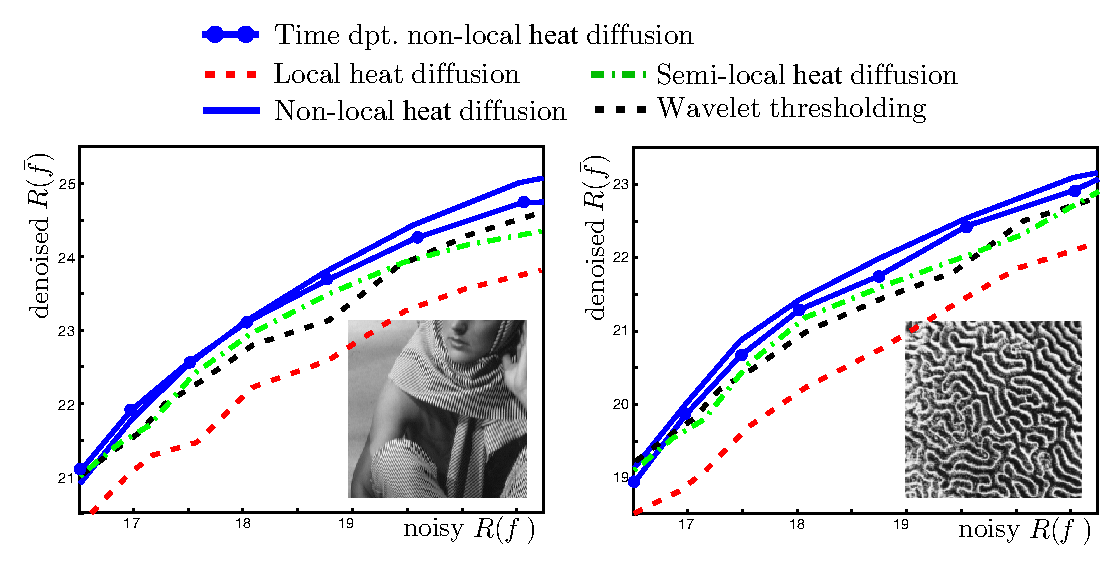
\includegraphics[width=\linewidth]{denoising/denoising-results-locality.eps}
}{
	Recovery error $R(\bar f)$ of local, semi-local and non-local estimators $\bar f$ for a natural image and a texture for various noise levels $R(\F)$.
%
}{fig-denoising-results-locality}

%%%%%%%%%%%%%%%%%%%%%%%%%%%%%%%%%%%%%%%%%%%%%%%%%%%%%%%%%%%
\subsection{Numerical Comparison of the Denoising Methods}
\label{subsect-numerical-comparison}

The numerical results compare the various algorithms in denoising situations with various noise levels. The tests are done on two images of $256 \times 256$ pixels, the first one (figure \ref{fig-denoising-results-locality}, left) contains smooth areas, edges and parallel stripes and the second one (figure \ref{fig-denoising-results-locality}, right) is a purely oscillating texture with complex patterns.


%%%%%%%%%%%%%%%%%%%%%%%%%%%%%%%%%%%%%%%%%%%%%%%%%%%%%%%%%%%
\paragraph{Comparison of the local and non-local kernels}

In order to study the advantages of using non-local computation over the more classical local and semi-local settings, we compare the denoising efficiency of the heat diffusion, exposed in section \ref{sect-heat-diffusion}. Figure \ref{fig-denoising-results-locality} shows a graphical comparison of the evolution of the recovery error $R(\bar f)$ with the noise level. We also report the results of the wavelet estimator, which constitutes a good benchmark. Figure \ref{fig-denoising-results-locality-visual} shows a visual comparison of the denoising methods for a noisy PSNR of 18.3dB. It is clear from these experiments that non-local methods tend to outperform both semi-local filterings and wavelet denoising. On more structured textures with periodic patterns such as the one on figure \ref{fig-denoising-results-visual}, the non-local technics perform even better. The time dependent heat flow, introduced in section \ref{sect-time-dpt-manifold}, does not seem to improve over a fixed manifold flow (such as the manifold heat equation). It is an open question to further understand the behavior of such a highly non-linear flow on images.

\myfigure{
\begin{tabular}{c c c} 
\includegraphics[width=0.27\linewidth]{denoising/corral/corral-original.png} &
\includegraphics[width=0.27\linewidth]{denoising/corral/corral-noisy.png} &
\includegraphics[width=0.27\linewidth]{denoising/corral/corral-denoise-wav.png} \\
Original & Noisy (18.3dB) & Wavelets (21.14dB) 
\end{tabular}
\vspace{1mm}\hfill
\begin{tabular}{c c c}
\includegraphics[width=0.27\linewidth]{denoising/corral/corral-denoise-local.png} &
\includegraphics[width=0.27\linewidth]{denoising/corral/corral-denoise-semilocal.png} &
\includegraphics[width=0.27\linewidth]{denoising/corral/corral-denoise-nonlocal.png} \\
Local (20.33dB) & Semi-local (21.39dB) & Non-local (21.76dB)\\[2mm]
\end{tabular}
}{
	Visual comparison of local, semi-local and non-local estimators for a noisy PSNR of $18.3dB$.
%
}{fig-denoising-results-locality-visual}




%%%%%%%%%%%%%%%%%%%%%%%%%%%%%%%%%%%%%%%%%%%%%%%%%%%%%%%%%%%
\paragraph{Comparison of the non-local denoising algorithms}

\myfigure{
\includegraphics[width=\linewidth]{denoising/denoising-results.eps}
}{
Risk $R(\bar f)$ of several estimators $\bar f$ for a natural image and a texture for various noise levels $R(\F)$.
%
}{fig-denoising-results}

Figure \ref{fig-denoising-results} compares the efficiency of the non-local denoising methods using the recovery error $R(\bar f)$. It shows that the estimators based on non-local graphs behave similarly, with a slight improvement for the threshold-based estimators. We note that in all the tests, the soft thresholding consistently performed better than the hard thresholding estimator.

Figure \ref{fig-denoising-results-visual} shows a visual comparison of the denoising methods for a noisy PSNR of $18.3$dB. One can notice the importance of normalizing the gradient operator as done in the estimator introduced in \ref{subsect-total-variation-graph}. The regularization with the un-normalized gradient tends to perform poorly over uniform areas where lots of patches share similar values and thus high values of $D(x)$ are expected. On this example, the thresholding operators give superior results and in particular the soft thresholding outperforms the non-local TV flow by 0.3dB. One should not however draw final conclusion from this image containing highly repetitive patterns. On more complex textures such as the one depicted on figure \ref{fig-denoising-results}, right, both methods give similar results.

\myfigure{
\begin{tabular}{c c}
\includegraphics[width=0.27\linewidth]{denoising/barb/barb-original.png} &
\includegraphics[width=0.27\linewidth]{denoising/barb/barb-noisy.png} \\
Original & Noisy (18.3dB) 
\end{tabular}
\vspace{1mm}\hfill
\begin{tabular}{c c c c}
\includegraphics[width=0.27\linewidth]{denoising/barb/barb-denoise-nonloc-gauss.png} &
\includegraphics[width=0.27\linewidth]{denoising/barb/barb-denoise-nonloc-quad.png}&
\includegraphics[width=0.27\linewidth]{denoising/barb/barb-denoise-nonloc-hard.png}\\
Heat (23.37dB) & Quadratic (23.22dB) & Hard (23.89dB)  \\[1mm]
\includegraphics[width=0.27\linewidth]{denoising/barb/barb-denoise-unorm-nonloc-tv.png} &
\includegraphics[width=0.27\linewidth]{denoising/barb/barb-denoise-nonloc-tv.png} &
\includegraphics[width=0.27\linewidth]{denoising/barb/barb-denoise-nonloc-soft.png} \\
TV Un-Norm. (21.72dB) & TV norm. (23.87dB) & Soft (24.16dB)\\[1mm]
\end{tabular}
}{
Risk $R(\bar f)$ of several estimators $\bar f$ for a natural image and a texture for various noise levels $R(\F)$. The soft and hard thresholding are applied over the non-local manifold spectral basis.
%
}{fig-denoising-results-visual}

\paragraph{Overall Comparison and Numerical complexity}

These experiments tend to support the following conclusions:
\begin{rs}
	\item Non-local methods gives superior results than semi-local ones in particular over repetitive patterns. 
	\item Iterative non-local algorithms (like heat-diffusion, section \ref{sect-heat-diffusion}, or quadratic regularization, section \ref{subsect-quad-regularization}) bring some  improvement over non-iterated methods like non-local means (section \ref{sect-noniterative-smoothing}) and wavelet thresholding \cite{mallat-book}. 
	\item Non-linear regularization like non-local TV (section \ref{subsect-total-variation-graph}) is slightly superior to quadratic regularization.
	\item Non-linear soft thresholding (section \ref{sec-thresholding}) is similar or better than non-local TV.
\end{rs}
It is however important to note that all of these improvements come with an important computational overhead. 

Iterative methods such as the manifold heat diffusion, section \ref{sect-heat-diffusion}, require typically of the order of 20 iterations to give satisfactory results and non-linear regularization such as manifold BV, section \ref{subsect-total-variation-graph}, requires even more iterations. Thus, These methods are much slower than a single filtering with non-local means. 

A major bottleneck of the spectral thresholding described in section \ref{sec-thresholding} with respect to the other approaches is the need to extract eigenvectors from the Laplacian operator. This can be somehow alleviated by applying the method to overlapping sub-blocks in the image and using sparse operators, as detailed in section \ref{sec-thresholding}. The main advantage of thresholding over PDE and regularization methods of sections \ref{sect-heat-diffusion-manifold} and \ref{sect-variational-regularization} is that it does not require to finely tune a stopping time or a regularization parameter $t$.

% kernel width $\si$. Similarly, the advantage with respect to non iterative filterings is that the choice of $\si$ is sensitive to noise level variations whereas the threshold is set automatically to approximately $3|\epsilon|$.



%%%%%%%%%%%%%%%%%%%%%%%%%%%%%%%%%%%%%%%%%%%%%%%%%%%%%%%%%%%
%%%%%%%%%%%%%%%%%%%%%%%%%%%%%%%%%%%%%%%%%%%%%%%%%%%%%%%%%%%
\subsection{Non-linear Approximation}

To further understand the superiority of the non-local denoising process, we exploit the connexion between non-linear estimation and approximation in an orthogonal basis. This property of orthogonal decomposition is used extensively to obtain minimax optimality results for thresholding estimators, see \cite{donoho-shrinkage}. Here we also exploit this feature of the spectral estimator to explore the behavior of non-local approximations and estimations. 

\paragraph{$M$-terms approximation}

The non-linear approximation of an image $f$ with $M$ coefficients in an orthogonal basis $\{u_\om\}_\om$ is written as
\begin{equation*}
	\label{eq-defn-nonlin-approx}
    f_M \eqdef \sum_{\abs{\dotp{f}{u_\om}}>T} \dotp{f}{u_\om} \, u_\om
    \qqwithqq
    M \eqdef \Card
    \enscond{\om}{\abs{\dotp{f}{u_\om}}>T},
\end{equation*}
The approximation error is then:
\begin{equation*}
    \norm{f - f_M}^2 = \sum_{\abs{\dotp{f}{u_\om}} \leq T} \abs{\dotp{f}{u_\om}}^2.
\end{equation*}
One wishes to use a basis $\{u_\om\}_\om$ that gives the best representation of data $f$ drawn from an image ensemble $f \in \Theta \subset \ldeux(\La)$. Optimizing the representation is then equivalent to maximizing the decay of the error $\norm{f - f_M}^2$ when $M$ increases, for all $f \in \Theta$. Asymptotically, one looks for bases $\{u_\om\}_\om$ such that $\norm{f - f_M}^2 = O(M^{-\al})$ for the largest possible $\al$.

\paragraph{Non-linear estimation and approximation}

Donoho and Johnstone \cite{donoho-shrinkage} proved that if the threshold is set to $T \eqdef |\epsilon|\sqrt{2\log(n)}$ then the decay of the average risk $E(\norm{\fz-\bar f}^2)$ is linked to the decay of the non-linear approximation in the basis $\{u_\om\}_\om$. More precisely they show that
\begin{equation}
	\label{eq-equiv-thresh-denoising}
	\norm{\fz-\fz_M}^2 \leq C_1 \, M^{-\al} \qquad\Longrightarrow\qquad
	E(\norm{\fz-\bar f}^2) \leq C_2 \, |\epsilon|^{\frac{2\al}{\al+1}}.
\end{equation}
where $C_1$ and $C_2$ are constants that depend only on $\fz$. This result is valid only for a fixed basis that does not depend on the noisy input $\F$. 

\paragraph{Extension to orthogonal dictionaries}

Results similar to \eqref{eq-equiv-thresh-denoising} can be proved for dictionaries of orthogonal bases such as the wavelet and cosine packets \cite{coifman-wavelet-packets} or the bandlets \cite{bandelets-siam}. Such a dictionary is written in abstract form as $\Dd = \{\Bb(\la)\}_{\la \in \Ga}$ where $\la$ is a parameter that specifies the orthogonal basis $\Bb(\la)$ of $\RR^n$ one wants to use to process a given function. In practice, one looks for a best basis $\Bb(\la^\star)$ in order to denoise or compress some input $f$. This is usually done by minimizing some Lagrangian cost function \cite{coifman-wavelet-packets} that enforces both good approximation in $\Bb(\la^\star)$ and sparsity of the expansion in $\Bb(\la^\star)$. In order for the equivalence \eqref{eq-equiv-thresh-denoising} between estimation and approximation to hold in this more general setting, one needs to have a control over the total number of basis vectors in the dictionary $\Dd$. Although the total number of bases $\#\Ga$ might grow exponentially with the dimension $n$, the total number of vectors has to grow only in a polynomial manner, i.e. 
\begin{equation}
	\label{eq-control-dictionary}
	\# \bigcup_{\la \in \Ga} \Bb(\la) \leq C n^{\beta}
\end{equation}
for some constants $C$ and $\be$, see \cite{krim-denoising,bandelets-denoising} for studies of denoising in a dictionary of orthogonal bases.

The spectral bases constructed in section \ref{subsec-spectral-basis} also form a dictionary $\Dd = \{\Bb(\Mm)\}_{\Mm \in \Ga}$ of orthogonal bases, where each $\Mm$ is a discrete manifold (either non-local or semi-local). In practice, it is difficult to control the number of such graphs $\#\Ga$ for a set of natural images. This number can be very large if one does not enforce strong constraints on the regularity of typical images, but the averaging implied by the width $\tau$ of the patch somehow alleviates this problem. Taking large patches is implicitly adding a strong regularization to the computation of the graph which avoids over-fitting and leads to good denoising performance. Our construction of adaptive non-local dictionaries thus does not come with constraint such as \eqref{eq-control-dictionary} but it is an important avenue for future work to explore the theoretical behavior of these estimators on realistic image models such as those considered below.

\paragraph{Theoretical bounds on non-linear approximation}

Equation \eqref{eq-equiv-thresh-denoising} shows that assessing the quality of the estimation process $\F \mapsto \bar f$ for the different kinds of orthogonal bases amounts to quantify the decay of the approximation error $\norm{f-f_M}^2$ for the images ensembles one would like to study. 
\begin{rs}
	\item For uniformly smooth images, both Fourier and wavelet bases behave similarly and the approximation error for a $\Cal$ image satisfies $\norm{f-f_M}^2 = O(M^{-\al})$. Since the semi-local and non-local basis vectors are in fact very similar to the Fourier vectors in this case, all the approximations behave similarly.
	\item A good model for images with regular edges is composed of images that are $\Cal$ outside a set of $\Cal$ edge curves, see \cite{donoho-wedglets}. This is close to the cartoon image model considered in section \ref{subsect-manifold-structure}. For this ensemble of geometric images, the Fourier expansion behaves baddly because of the presence of step discontinuities and satisfies $\norm{f-f_M}^2 = O(M^{-1/2})$. In contrast, the wavelet expansion is able to make use of the bounded total variation of such a function and its error satisfies $\norm{f-f_M}^2 = O(M^{-1})$, see \cite{mallat-book}. This is however sub-optimal and other bases such as wedgelets \cite{donoho-wedglets}, curvelets \cite{candes-tight-frame} and bandlets \cite{bandelets-siam,bandelets-peyre} are able to improve this approximation rate by exploiting the regularity of edge curves. One might expect that non-local adapted bases also capture this asymptotic decay of the error, thus providing an optimal tool to denoise cartoon images.
	\item A simple model for turbulent textures is an oscillating function with locally parallel level sets. Such a function can be written as $f(x) = \cos(\Phi(x))$ where $\Phi$ is a slowly varying phase function, see \cite{demanet-waveatoms}. For this ensemble of locally parallel textures, the wavelets expansion fails to capture the oscillating regularity. Oscillating atoms such as the wave atoms \cite{demanet-waveatoms} are able to capture such a behavior and enjoy a better approximation rate. Non-local processing methods also seems to perform well on these locally parallel textures, as shown on figure \ref{fig-denoising-results-locality-visual}.
	%  and its error decay is like $\norm{f-f_M} = O(M^{-1/2})$  of $\norm{f-f_M} = O(M^{-1/2})$
	\item For more complex images ensembles containing textures, there is no available scheme with provable approximation rate. Non-local denoising algorithms seems however to process efficiency several kinds of repetitive texture patterns \cite{buades-nl-means}. 
\end{rs}

In the following we perform a numerical estimation of the approximation rate in order to have information on the relative efficiency of processing methods.

\paragraph{Numerical estimation of the approximation error}

Although our non-local dictionary of spectral bases does not satisfy the polynomial grow \eqref{eq-equiv-thresh-denoising}, we use the approximation error $\norm{f-f_M}$ as a measure of the efficiency of this adaptive estimation scheme. In order to have a fair comparison, the non-local bases are computed from a noisy image $f+\epsilon$. The noise level $|\epsilon|^2$ is set to $n^{-1}\norm{f-f_M}^2$ where $f_M$ is the $M$-terms approximation of $f$ in the wavelet basis.

Figure \ref{fig-approx-error-decay} shows the approximation error $\norm{f-f_M}^2$ of $f$ in various orthogonal bases. It is important to remember that the adapted basis for the semi-local and non-local Laplacians are estimated from a noisy observation $\F+\epsilon$ and not from the original image $f$ that is not available in a denoising scenario. One can see that the non-local approximation is consistently better than the other approximation schemes. This reveals the superiority of non-local denoising methods to process images whose structures are not well captured by classical expansions such as Fourier or wavelets. Note however that both the semi-local and the non-local expansions are not suitable for applications to image compression since the adapted basis $\{u_\om\}_\om$ is not available for the decoder.

\myfigure{
\raisebox{1cm}{ % 
\includegraphics[width=0.26\linewidth]{approximation/barb-original.png} }
\qquad
\includegraphics[width=0.5\linewidth]{approximation/barb-approx-err-decay.eps}
}{
Left: original image $f$. Right: error decay $\log_2(\norm{f-f_M})$ of the approximation $f_M$ of $f$ with $M$ coefficients (expressed in \% of the total number of coefficients) in various orthogonal bases.%
}{fig-approx-error-decay}

\section*{Conclusion}

This article reviewed several recent approaches to image estimation using a regularizer computed on a discrete manifold. This allows one to consider both local, semi-local and non-local methods in an unifying framework. The spectral bases associated to the Laplacians on these discrete manifolds define adaptive orthogonal decompositions that are exploited to build non-linear thresholding operators. The numerical experiments show that this new class of estimators performs at least as good as state of the art diffusions and regularizations on non-local graphs. It also enables an exploration of semi-local and non-local methods using approximation in adaptive orthogonal bases.


\bibliographystyle{siam}  % plain alpha
\bibliography{bibliography}

\end{document}
